% clase de documento
\documentclass[a4paper,11pt]{report}
%
\linespread{1.3}
%
%--------------------   start of the 'preamble'
%
% packages para el documento
%
\usepackage[hyphens]{url}
\usepackage{graphicx,amssymb}                  %amssymb:para simbolos matematicos%
\usepackage{rotating}          %para poder poner fotos apaisadas%
\usepackage[pdftex]{hyperref, color}
\usepackage{amscd}
\usepackage{amsmath}                           %para escritura matematica%
\usepackage{xy}
\usepackage[papersize={180mm,250mm}]{geometry} %dimesiones del documento%
\usepackage{array}                             %per canviar mides en taules
\usepackage{bm}
%\usepackage[pdftex]{color,graphicx}           %para links
\usepackage[pdftex]{hyperref, color}
\usepackage{eepic} %primera lletra gran



%
\hypersetup{pdfpagemode={UseOutlines},colorlinks=true,pdftitle=FAULTS manual ,
pdfauthor=Montse Casas Cabanas,pdfstartview=FitH,pdfkeywords=(manual)}
%
%
%---------------------   end of the 'preamble'
%
%
\begin{document}  
\sloppy %\makes Latex less fussy for line breaking (for urls)
%-----------------------------------------------------------
\title{\Huge\bf FAULTS manual}
\author{Montse Casas Cabanas (CIC energiGUNE), Marine Reynaud (CIC energiGUNE) \\
Jokin Rikarte Ormazabal (CIC energiGUNE), Pavel Horbach (ILL) \\
and Juan Rodriguez Carvajal (ILL)}
\date{September 2018}
\maketitle
%-----------------------------------------------------------
\pagenumbering{roman}
\tableofcontents
%-----------------------------------------------------------
\chapter{The FAULTS program}
\label{faults}
\pagenumbering{arabic}
\setcounter{page}{1}


FAULTS is a Fortran90 program to refine X-ray Powder Diffraction (XRD) and Neutron Powder Diffraction (NPD) patterns of crystal systems with any type of coherent planar defect.
This program is based on the DIFFaX program \cite{DiffaxPaper,DiffaxDownload} and on the library CrysFML (Crystallographic Fortran Modules Library)  \cite{CrysFMLPaper,CrysFMLDownload}. \\

The DIFFaX program (Diffracted Intensities From Faulted Xtals) calculates diffraction intensities from defective layered crystals.
This tool has been widely used to interpret the diffraction data of one-dimensionally disordered systems and it is based on an algorithm that exploits the recursive nature of the patterns found in randomized stacking sequences to compute the average interference wavefunction scattered from each layer type occurring in a faulted crystal (mathematical details can be found in references \cite{DiffaxMaths,Hend1942}). However, approximate or merely qualitative results sometimes are not sufficient for a thorough microstructural characterization, a computerized comparison of the DIFFaX calculated intensities with experimental data has been developed.
The resulting code is the FAULTS program \cite{FAULTSPaper1,FAULTSPaper2}.   Note that FAULTS, as DIFFaX, can also simulate 2D diffraction patterns and diffuse streaks in reciprocal space for single crystals.\\

The program  is distributed in the hope that it will be useful, but without any warranty of being free of internal errors. The authors acknowledge all suggestions and notification of possible bugs found in the program.\\


\section{Download and installation}

FAULTS can be obtained either as part of the FullProf Suite \cite{FPDownload, FPPaper, FPManual} at \url{www.ill.eu/sites/fullprof/}, for Windows, Linux or MacOS, or as a separate program for Windows by downloading the compressed file FAULTS.zip at \url{www.cicenergigune.com/en/areas-investigacion/power-storage-batteries-and-supercaps/lineas-investigacion/li-ion/faults/}.\\


In case the user chooses to install FAULTS with the FullProf Suite, the program FAULTS can be launched directly from the FullProf Suite Toolbar or by opening a terminal and invoking the program as: Faults myinputfile.flts.
If FAULTS is downloaded as a separate Windows program, it should be launched from a command-line window (cmd.exe), after having copied the standard scattering factor data file \textit{data.sfc} into the working folder.


\section{Program specifications}


Conventionally, crystals are thought in terms of unit cells, atoms in the asymmetric unit and a determined symmetry space group. Nevertheless, to use FAULTS, as in the case of DIFFaX \cite{DiffaxManual}, one needs to think of crystals in terms of atomic sheets, or layers, which can be interconnected via stacking operations occurring with a
certain probability. By means of this description, planar defects can be described as different layer types and/or
transition vectors. Frequently, the plane of layers will not coincide conveniently with any of
the unit cell faces of the parent crystal. Then, a transformation of atom coordinates to a
new cell system is required.\\

The structural information as well as the refinement details are read by FAULTS from a free format input data file, with \textit{.flts} extension.
Each value used to describe the structure is associated to a refinement
code that allows the possibillity of restrictions. The user must be aware of the way he(she) can control the refinement procedure:
the number of parameters to be refined, fixing parameters, making constraints, etc.
The experimental XRD or NPD patterns can be read from many different formats and background subtraction can be achieved by
linear interpolation or polynomially after applying the scale factor. Impurities or other phases are treated as background as well, and their pattern information must be given by the user.
Another major feature of FAULTS is the implementation of a more adequate isotropic size broadening treatment which takes
into account the Gaussian  and Lorentzian  contributions to the FWHM in addition to the consideration of a finite
number of layers per crystallite already present in DIFFaX \cite{DiffaxPaper,DiffaxDownload,DiffaxManual}.
The refinement is carried out using a Levenberg Marquardt fit.
The quality of the agreement between observed and calculated profiles is given by the R-Factor and Chi$^{2}$ agreement factors that are calculated at the end of each refinement cycle and are defined as follows:

Profile factor:

$$Rp = 100 \frac {{\sum_{i=1,n}}{ \mid y_{i} - y_{ic} \mid }} {\sum_{i=1,n} y_{i}}$$

\vspace{0.5cm}
\noindent where $y_{i}$ is the profile intensity and $y_{ic}$ is the number of calculated counts at the \textit{i}th step.

Reduced Chi square:

$$Chi^{2}= \left[ \frac{R_{wp}}{R_{exp}}\right]^{2}$$

\vspace{0.5cm}
\noindent being $R_{\omega p}$ and $R_{exp}$ the Weighted Profile Factor and the Expected Weighted Profile Factor respectively, which are defined as:

$$R_{wp}=100\left[\frac{\sum_{i=1,n}{w_{i}\mid y_{i} - y_{ic} \mid^{2}}}{\sum_{i=1,n}{w_{i}y_{i}^{2}}}\right]^{1/2}$$

\vspace{0.5cm}
\noindent and

$$R_{exp}=100\left[\frac{n-p}{\sum_{i}{w_{i}y_{i}^{2}}}\right]^{1/2}$$

\vspace{0.5cm}
\noindent where \textit{n-p} is the number of degrees of freedom and $w_{i}=1/\sigma_{i}^{2}$, with $\sigma_{i}^{2}$ referring to the variance of the ``obserbation" $y_{i}$.



\section{Input files}

\subsection {The input control file:  \textbf{CFILE.flts}}


The input control file is a free format file that contains all the structural
data and the type of calculation to be done. This file must be written by the user.\\

The FAULTS input file is similar to the one used in DIFFaX \cite{DiffaxManual}, although there are some differences that should be taken into account to avoid errors. The DIFFaX2FAULTS convertor, which permits to convert DIFFaX input files into FAULTS ones, is available at \url{www.cicenergigune.com/en/areas-investigacion/power-storage-batteries-and-supercaps/lineas-investigacion/li-ion/faults/}.\\  


Free format means that the input file is not case sensitive and that the different sections do not have to follow a concret sequence, however,
a space is needed between each item and all the section headings and subsection keywords must be present. Each line must not exceed 132 characters, taking into account the blank spaces.
When the program is run, mistakes will normally generate error messages.
 Empty lines as well as lines starting with the exclamation symbol (\emph{!}) in the first column are considered as comments
and are ignored by the program. Also, comments can be placed at the end of a line if they are in braces ($\{\}$). It is recommended not to use tabulator to introduce blank spaces when editing the file, as some editors do not consider it as blank spaces.\\

An example of input control file can be found in figures   \ref{control1}, \ref{control2} and \ref{control3}. The different section headings that
constitute the input control file appear in orange color, comments appear in italics (and of course after a \emph{!} symbol), subsection keywords in red, parameters in blue and refinement codes in green.
The latter are codewords that allow the control of the refined parameters. As in the FullProf program \cite{FPPaper,FPManual}, these are the numbers C$_x$ that are
entered for each refined parameter.  A zero codeword means that the parameter is not being refined.
For each refined parameter, the codeword is formed as:

$$ C_x= sign (a) (10p + |a| )	$$

\vspace{0.5cm}
\noindent where \emph {p} specifies the ordinal number of the parameter  \emph{x} and \emph {a} is the factor by which the computed shift (the parameter variation in each refinement cycle)
will be multiplied before use.\\

Below, each section, which has to begin with the corresponding heading, is explained in more detail.


\begin{figure}[p]
\begin{center}
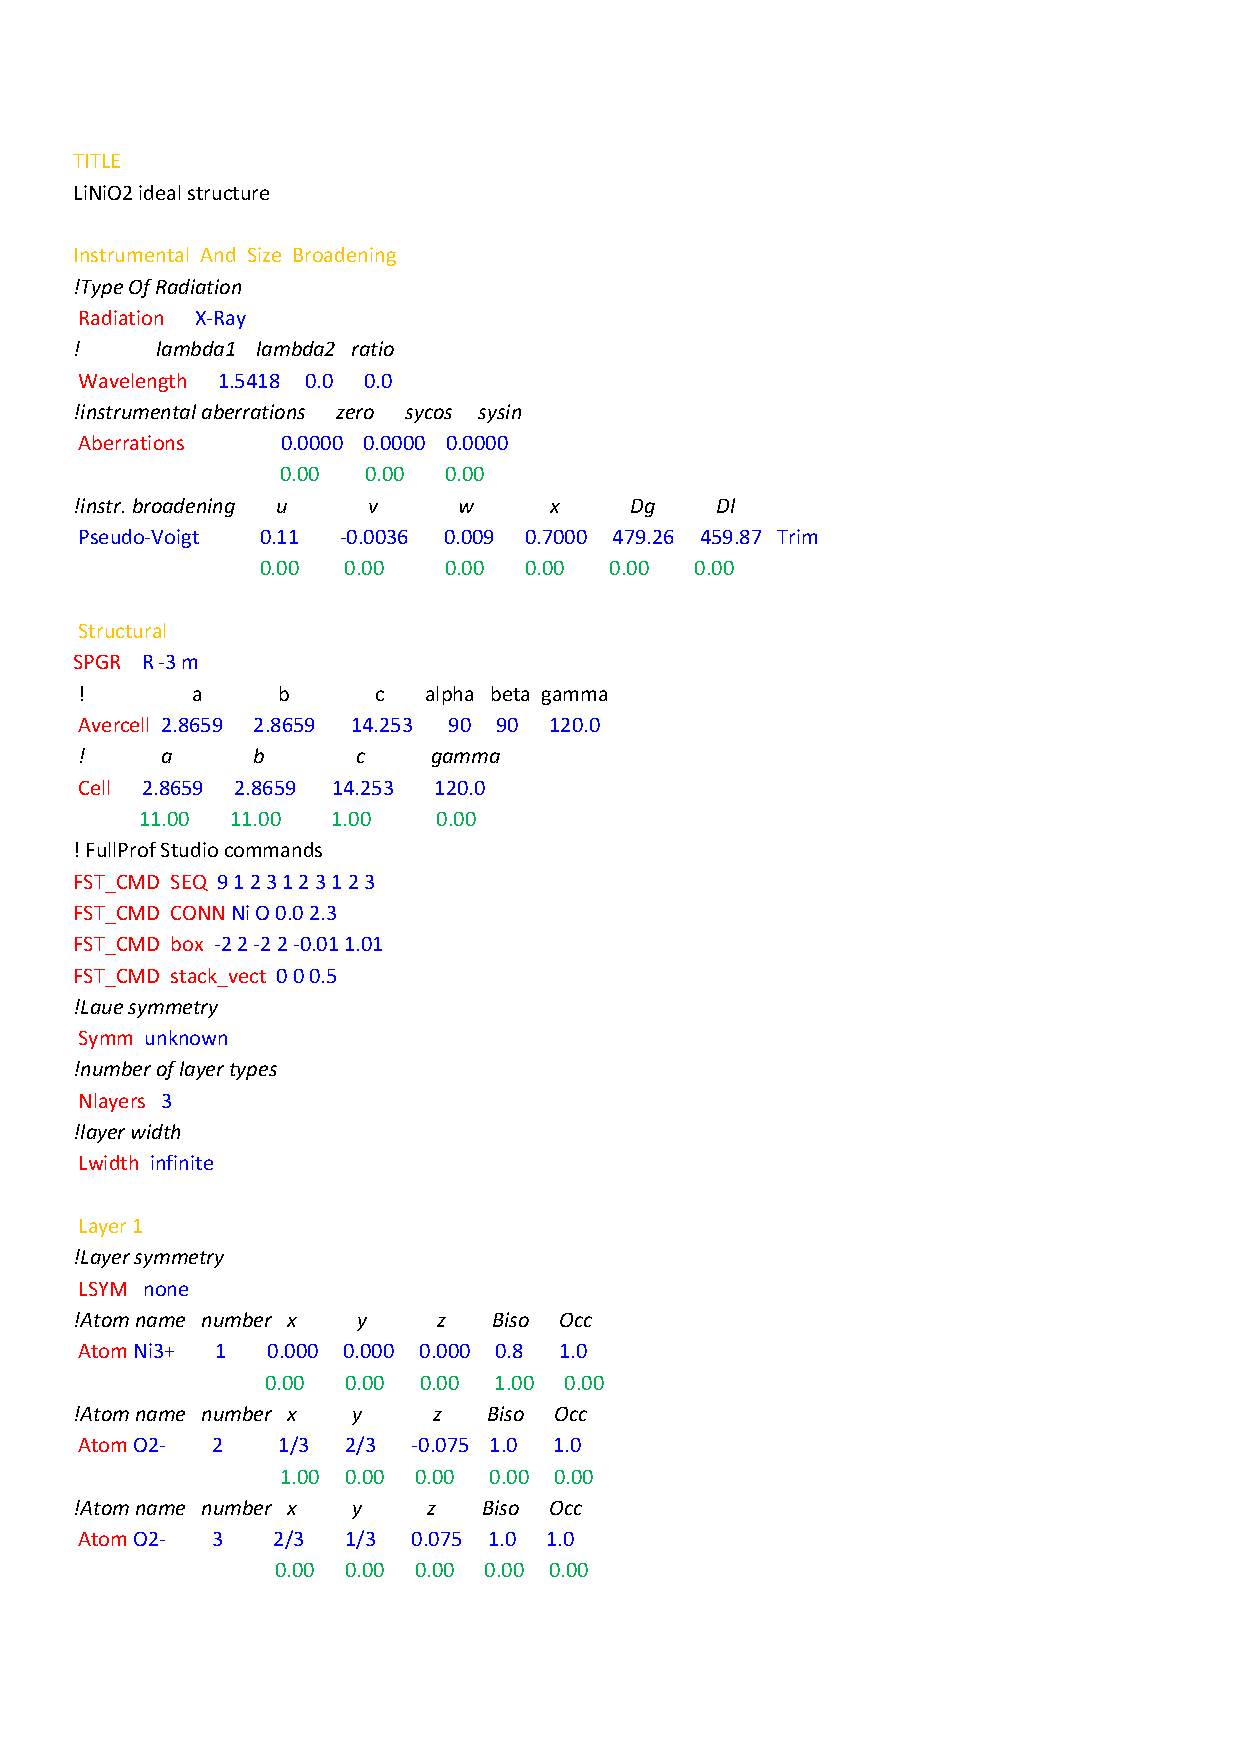
\includegraphics [width=5.5 in]{control1.pdf}
\caption{\bf Example of input control file, corresponding to the ideal structure of $LiNiO_{2}$.}
\label{control1}
\end{center}
\end{figure}

\begin{figure}[p]
\begin{center}
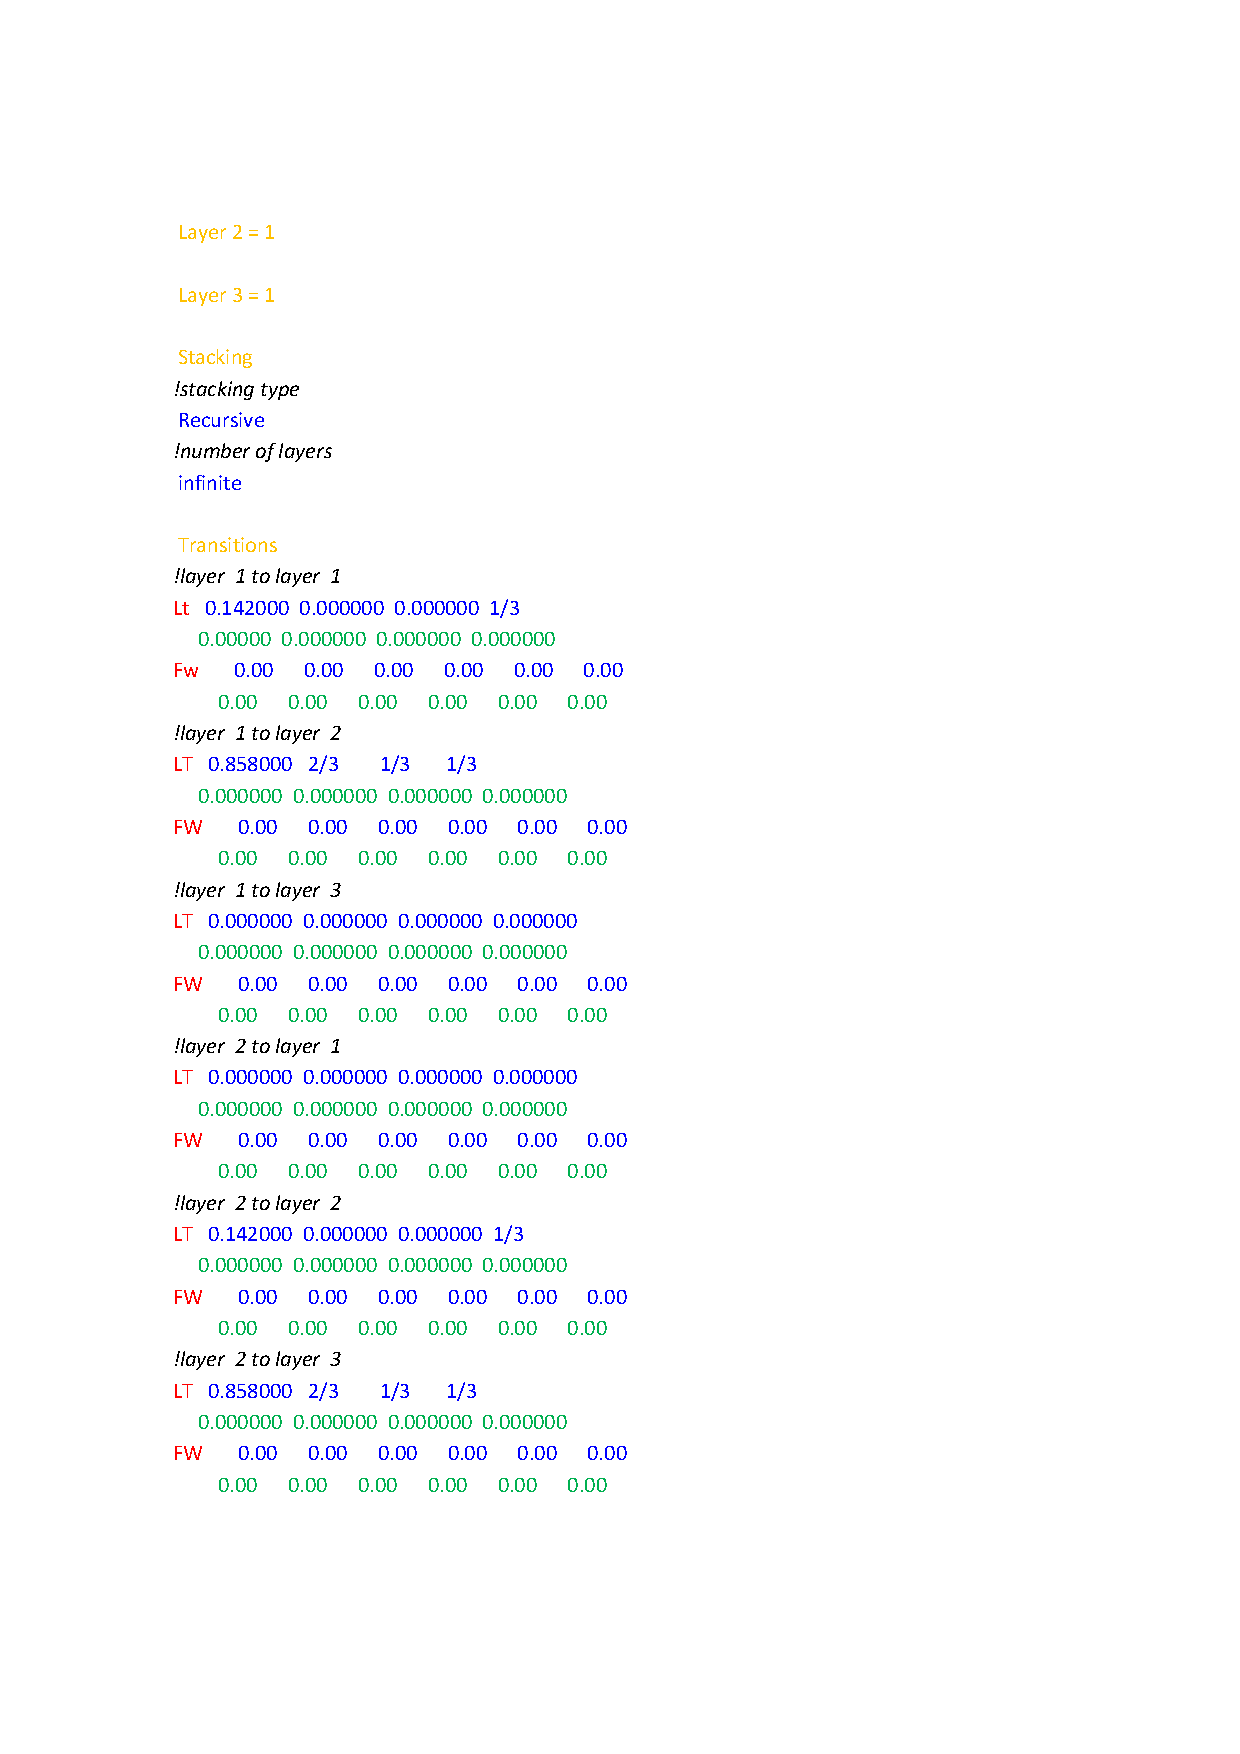
\includegraphics [width=5.5 in]{control2.pdf}
\caption{\bf Cont. Example of input control file, corresponding to the ideal structure of $LiNiO_{2}$.}
\label{control2}
\end{center}
\end{figure}

\begin{figure}[p]
\begin{center}
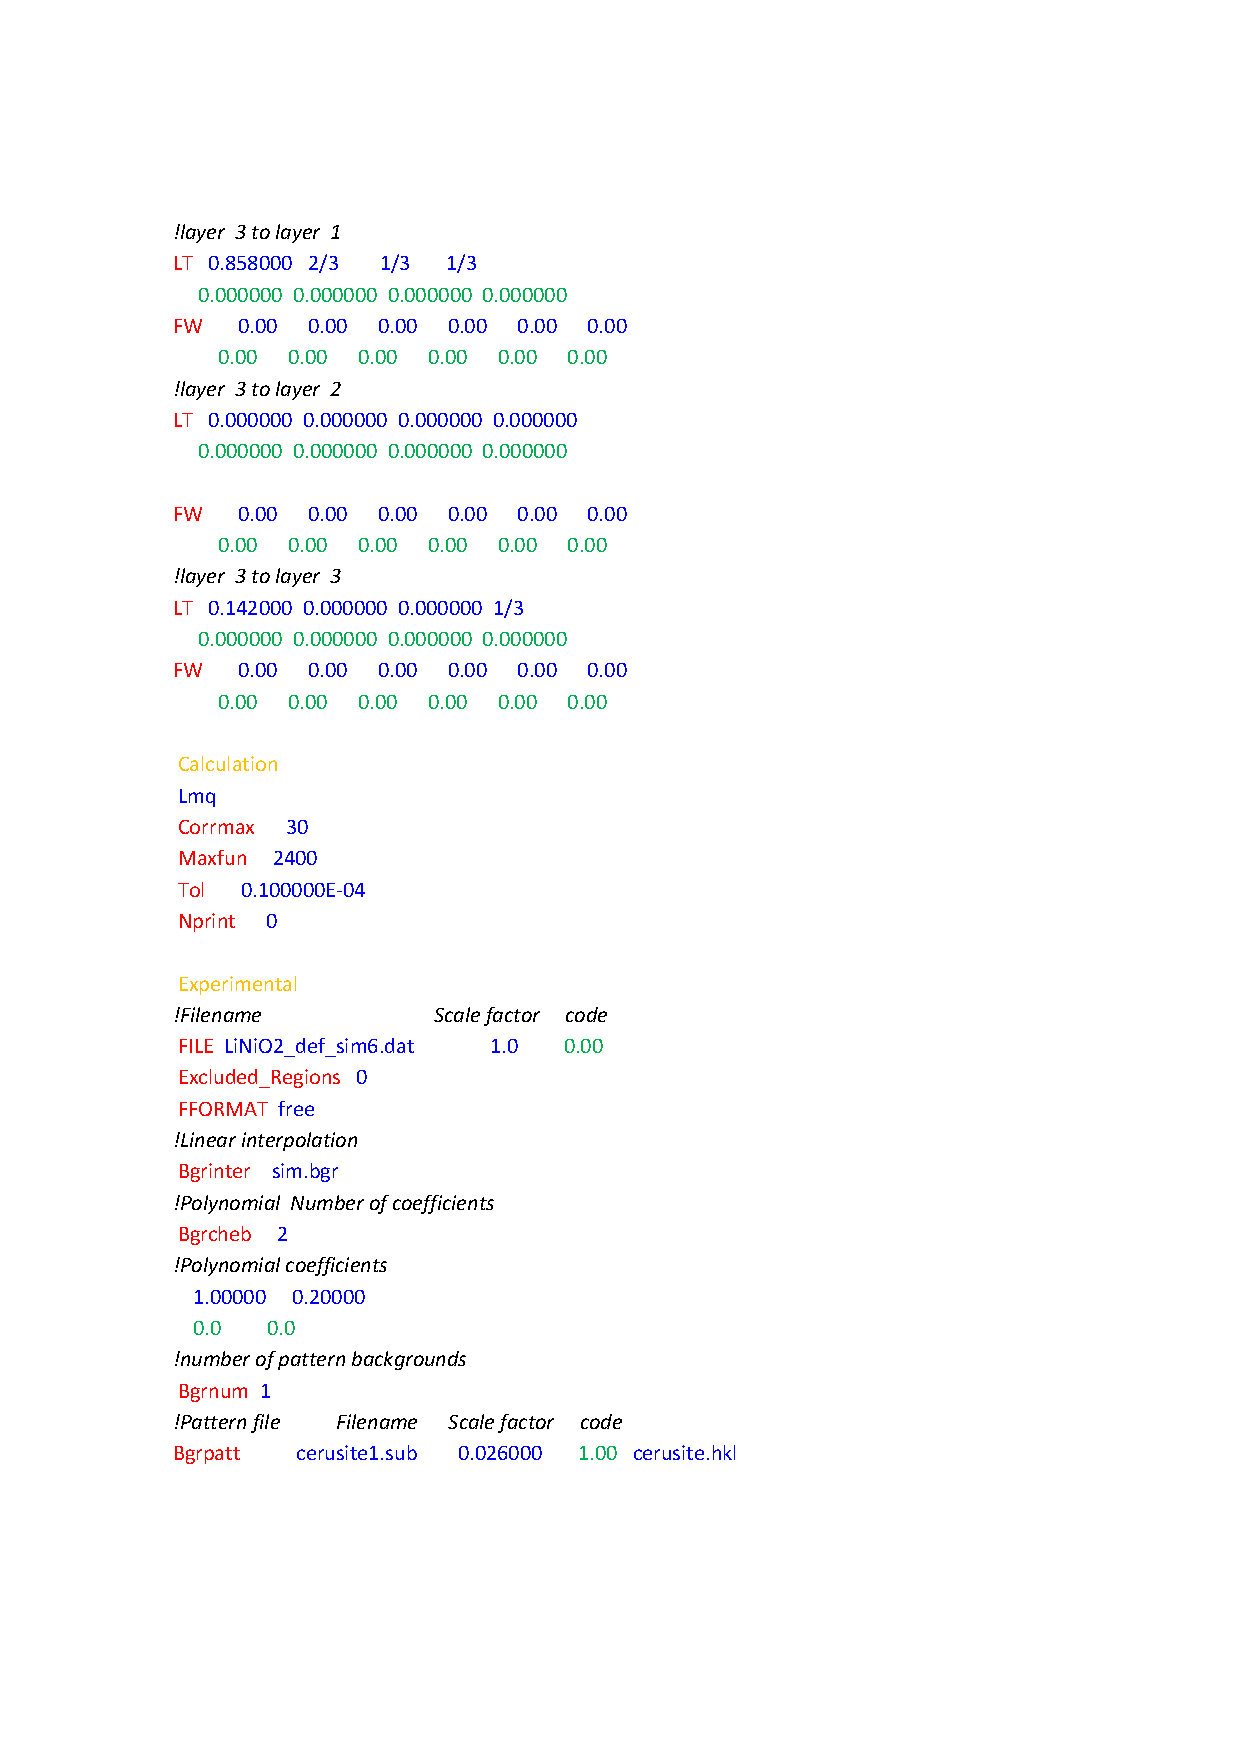
\includegraphics [width=5.5 in]{control3.pdf}
\caption{\bf Cont. Example of input control file, corresponding to the ideal structure of $LiNiO_{2}$.}
\label{control3}
\end{center}
\end{figure}

\subsubsection{ \emph{Title} section}

The document must begin with this section. TITLE heading must be followed in the next line by the title chosen by the user.

\subsubsection{ \emph{Instrumental and size broadening} section}

The first line must contain the heading INSTRUMENTAL AND SIZE BROADENING. The data that follow describe
the type of radiation and the instrumental conditions as well as the parameters needed for size broadening, which are refinable parameters.
To refine the parameters that constitute this section it is not necessary to recalculate the diffraction pattern in each cycle,
 so, for computational economy it is strongly recommended to refine them separately.\\

\begin{itemize}
\item \textbf{Radiation type:} The line must begin with the keyword \textit{radiation}, followed by one of the different three options, which are  X-RAY, NEUTRON and ELECTRON (the latter for the simulation of selected area diffraction patterns -SADP-).
\item \textbf{Wavelength:}  In addition to $\lambda_{1}$,  FAULTS reads also the value of $\lambda_{2}$
and the intensity ratio  ${I_2}/ {I_1}$ (although in the case of monochromatic radiation it is only necessary to introduce $\lambda_{1}$).
$\lambda$ unit is \AA \thinspace and this line must begin with the keyword \textit{wavelength}.
\item \textbf{Aberrations:} Keyword \textit{aberrations} followed by values for the instrumental aberrations (zero, sycos and sysin) must be given. As they are refinable, refinement codes must be entered in the next line.
The parameters sycos and sysin relate to systematic 2Theta shifts having a $cos{\theta}$  and $sin{\theta}$ dependency, respectively, that originate from different physical and/or geometrical problems depending on the
diffraction geometry (see FullProf manual for more details \cite{FPManual}).


\item \textbf{Profile parameters:} Instrumental and size broadening are treated differently than in DIFFaX.
In both cases, the calculated pattern is convoluted with a profile function (indicated by the keyword \textit{Gaussian}, \textit{Lorentzian} or \textit{Pseudo-Voigt}) that takes into account both instrumental and size effects.
The FWHM of the Gaussian ($H_{G}$) and Lorentzian ($H_{L}$) components of the peak profile have an angular dependence given by: \label {FWHM}

$$ H_{G}^{2} = U tan^{2}{\theta}+ V tan {\theta} + W + \frac{4ln2\lambda^{2}}{\pi D_{G}^{2} cos^{2} {\theta}} (\frac {180}{\pi})^2$$

$$ H_{L} = X tan {\theta} + \frac{2 \lambda}{\pi D_{L} cos \theta} (\frac {180}{\pi})$$


U, V, W and X, which must be introduced by the user, are refinable parameters that constitute the instrumental resolution function (IRF). It is always advisable to know their values a priori
and fix them during the refinement (although U and X can be refined to account for strains).
They must be followed by $D_{G}$ and $D_{L}$, which are the parameters that are used to model the isotropic size broadening due to a finite size of the crystallites ( $\leq $ 1  $\mu$m). They are also refinable.
If the sample is not affected by size broadening,  $D_{G}$ and $D_{L}$ can take any value $\geq $ 5000 \AA.

\item \textbf{TRIM keyword:} As in DIFFaX \cite{DiffaxManual}, the optional keyword \textit{trim}, which has to be put in the same line as the profile parameters, tells the program to ignore intensity information
close to the origin when simulating the instrumental broadening for a powder diffraction
pattern. The peak at the origin is usually many orders of magnitude more intense than
any other peak of the diffraction pattern, and the background that is generated by the tail of this
peak, when broadened, can easily swamp peaks close to the origin. When \textit{trim} is specified,
the unbroadened pattern that is written to file retains the data at the origin, whereas
the broadened data that is written to file suppresses the peak at the origin. It is generally
desirable to specify \textit{trim} whenever the powder pattern angular range includes the origin.
\textit{trim} has no effect if the powder pattern angular range requested by the user does not include
the origin.
\end{itemize}

\subsubsection{\emph{Structural} section}

This section must begin with a first line containing the heading STRUCTURAL.
\begin{itemize}
\item \textbf{Cell parameters:} The keyword which this line has to begin with is \textit{cell}. The value of \textbf{c}, perpendicular to the a-b plane (and therefore
parallel to the stacking direction), is needed to provide a reference scale along the stacking
direction with which to define the z-component of the stacking vectors. \textbf{c} does not have
to correspond to any special periodic dimension along the stacking direction for any of the
layers. However all the layers must share the same dimensions, \textbf{a}, \textbf{b} and $\gamma $.
These are all refinable parameters and the units are \AA \thinspace for \textbf{a, b} and \textbf{c}, and degrees for $\gamma$.\newline

 \item \textbf{Laue symmetry:} In this case the keyword is \textit{symm}. There are 12 options : \textbf{-1, 2/M(1) , 2/M(2), MMM, -3, -3M, 4/M, 4/MMM, 6/M, 6/MMM, AXIAL} and \textbf{UNKOWN}.
Axial constraints the program to integrate only along 00\emph{l}  (useful in turbostratic structures) and if UNKNOWN is specified
the program will establish the symmetry by randomly sampling the reciprocal space. In this case, the user can specify a percentage of tolerance on intensity deviations for this search. Otherwise the program tests the user option and, if it is not consistent with the cell parameters, it is automatically changed.

 \item \textbf{Number of layer types: }The keyword is \textit{nlayers}. It is the number of different layer types needed to describe the structure. If two layers are structurally identical but
 their stacking vectors are  different, they are considered as two different layer types.

 \item \textbf{Layer caracteristic width: } Unlike in DIFFaX, this line is compulsory, and it must begin with the keyword \textit{lwidth}. Then the layer characteristic width is especified, in \AA.
There are two possible formats for this line: width along \textit{a} and width along \textit{b}, both refinable values, or \textit{infinite}. For example,


\begin{flushleft}
\begin{tabbing}
	\hspace*{1.5 cm}!layer width\\*
	\hspace*{1.5 cm}Lwidth  \=120.00   \=300.00 \\*
	\hspace*{1.5 cm}				\>0.0      \>0.0
\end{tabbing}	
\end{flushleft}

or

\begin{flushleft}
\hspace*{1.5 cm}!layer width\\*
\hspace*{1.5 cm}Lwidth   infinite	
\end{flushleft}


\item \textbf{Optional generation of the Bragg positions of the average cell:}
In case the cell parameters defined for the FAULTS refinement are different from the original cell (the cell from which the disordered model comes from; for instance, in the case of a monoclinic or triclinic average cell), the user can ask the program to generate the Bragg positions corresponding to the average cell in the output file CFILEn.prf (see section \ref{prff}).
To do so, the user has two options:\\
(1) either he(she) indicates manually the space group (after the keyword \textit{SPGR}) and the cell parameters \textit{a}, \textit{b}, \textit{c}, $\alpha$, $\beta$, $\gamma$ (after the keyword \textit{Avercell}) of the average cell by adding the following optional lines in the \textit{Structural} section:

\begin{flushleft}
\begin{tabbing}
	\hspace*{1.50 cm}!Average cell parameters (for Bragg positions in .prf file)\\*
	\hspace*{1.50 cm}Avercell \=3.12 \=4.15  \=4.60   \=90.00 \=118.79 \=90.0 \\*
	\hspace*{1.50 cm}!Average space group (for Bragg positions in .prf file)\\*
	\hspace*{1.50 cm}SPGR \=C 2/m
\end{tabbing}	
\end{flushleft}

(2) or, by means of the keywords \textit{CalcAverCell} and \textit{SPGR}, he(she) asks the program to calculate the average cell from a sequence of layers that he(she) specifies with the following optional lines in the \textit{Structural} section:

\begin{flushleft}
\begin{tabbing}
	\hspace*{1.50 cm}!Number of stacking vectors needed to calculate the average cell\\*
	\hspace*{1.50 cm}CalcAvercell \=2 \\*
	\hspace*{1.50 cm}!Specific sequence to calculate the average cell\\*
	\hspace*{1.50 cm} \=1 2 \\*
	\hspace*{1.50 cm}!Average space group (for Bragg positions in .prf file)\\*
	\hspace*{1.50 cm}SPGR \=C 2/m
\end{tabbing}	
\end{flushleft}

Note that the average cell parameters and space group are only used for the Bragg positions calculation for the .prf file and are not taken into account for the pattern calculation during the refinement or simulation.

\item \textbf{Optional commands for generation of a .CIF file and visualization of the structure with FullProf Studio and VESTA:} To simplify the construction of the structural section and to avoid errors, it is recommended to regularly draw the structure with the help of a visualization program, such as FullProf Studio \cite{FPSDownload,FPSManual} or VESTA \cite{VESTApaper,VESTAwebsite}. For this, the program describes the stacking of layers in a big artificial box containing all the atoms of the layers that are asked to be painted by the user. 
To do so, the user should ask the program to generate additional the output files \textit{.fst}, \textit{.cif} and \textit{.vesta} (see section \ref{fstf}) suitable for FullProf Studio and VESTA, respectively , by entering an optional line beginning with the keyword \textit{FST\_CMD}, followed by the keyword \textit{SEQ}, the number of layers and the sequence of the layers to be drawn; for example:

\begin{flushleft}
\begin{tabbing}
	\hspace*{1.50 cm}!FullProf Studio commands \\*
	\hspace*{1.50 cm}FST\_CMD \=SEQ  \=5  \hspace*{0.30 cm}1 1 2 3 1
\end{tabbing}	
\end{flushleft}

Then the user can add as many optional lines as needed, each of them beginning with the keyword \textit{FST\_CMD}, followed by the required FullProf Studio commands (see the FullProf Studio manual for more details \cite{FPSManual}). For example, to control respectively the drawing of Ni-O bonds (of length between 0.0 and 2.3 \AA) polyhedra of the example input file, the limits of the box and the position of the first layer in the artificial box, the user may add the following lines:

\begin{flushleft}
\begin{tabbing}
	\hspace*{1.50 cm}FST\_CMD  \=CONN \hspace*{0.20 cm}Ni O \hspace*{0.20 cm}0.0 2.3\\*
	\hspace*{1.50 cm}FST\_CMD  \>BOX  \hspace*{0.20 cm}-2.0 2.0 \hspace*{0.20 cm}-2.0 2.0 \hspace*{0.20 cm}-0.01 1.01 \\*
	\hspace*{1.50 cm}FST\_CMD  \>stack\_vect  \hspace*{0.20 cm}0 0 0.5
\end{tabbing}	
\end{flushleft}

\end{itemize}

\subsubsection { \emph{Layers} section}

\begin{itemize}
\item \textbf{Layer number:} The layers have to be described with the header \emph{LAYER} followed by the ordinal corresponding number. If two layers are structurally identical
it will be enough to write \emph{LAYER j = i}  where \emph{i} and \emph{j} are the ordinal numbers that correspond to each layer (a blank space is necessary between the number of layer and the \emph{=} symbol). Then, for layer \emph{j} the rest of the section can be avoided.

\item \textbf{Layer symmetry:} The keyword \textit{lsym} must be followed by one of the two options: \textbf{NONE} or \textbf{CENTROSYMMETRIC}. If the latter is specified,
only the asymmetric half of the atom coordinates
need to be entered, and the program will create another identical atom in (-x,-y,-z) per each atom described in the layer. Take care to halve the occupancy in case of the atoms located at any inversion center.

\item \textbf{Atomic data:} For each atom the keyword \textit{atom} must be written, followed by a specific 4 characters name. The first two characters correspond to the atomic symbol and the last two represent the valence.  If the symbol has only one character, contrary to DIFFAX, there must not be a space between the symbol and the charge (Ex. \mbox{F1-}, \mbox{Ni2+}). Some atoms do not require any valence (ex. C). Below is the list of the names accepted by FAULTS (this list is found in the standard scattering factor data file \textit{data.sfc}): \\
% In case of doubt, the user can check the correct form in the file \textit{data.sfc}. \\
H ; H. ; D ; H1- ; He ; Li ; Li1+ ; Be ; Be2+ ; B ; C ; C. ; N ; O ; O1- ; O2- ; F ; F1- ; Ne ; Na ; Na1+ ; Mg ; Mg2+ ; Al ; Al3+ ; Si ; Si. ; Si4+ ; P ; S ; Cl ; Cl1- ; Ar ; K ; K1+ ; Ca ; Ca2+ ; Sc ; Sc3+ ; Ti ; Ti2+ ; Ti3+ ; Ti4+ ; V ; V2+ ; V3+ ; V5+ ; Cr ; Cr2+ ; Cr3+ ; Mn ; Mn2+ ; Mn3+ ; Mn4+ ; Fe ; Fe2+ ; Fe3+ ; Co ; Co2+ ; Co3+ ; Ni ; Ni2+ ; Ni3+ ; Cu ; Cu1+ ; Cu2+ ; Zn ; Zn2+ ; Ga ; Ga3+ ; Ge ; Ge4+ ; As ; Se ; Br ; Br1- ; Kr ; Rb ; Rb1+ ; Sr ; Sr2+ ; Y ; Y3+ ; Zr ; Zr4+ ; Nb ; Nb3+ ; Nb5+ ; Mo ; Mo3+ ; Mo5+ ; Mo6+ ; Tc ; Ru ; Ru3+ ; Ru4+ ; Rh ; Rh3+ ; Rh4+ ; Pd ; Pd2+ ; Pd4+ ; Ag ; Ag1+ ; Ag2+ ; Cd ; Cd2+ ; In ; In3+ ; Sn ; ; Sn2+ ; Sn4+ ; Sb ; Sb2+ ; Sb5+ ; Te ; I ; I1- ; Xe ; Cs ; Cs1+ ; Ba ; Ba2+ ; La ; La3+ ; Ce ; Ce3+ ; Ce4+ ; Pr ; Pr3+ ; Pr4+ ; Nd ; Nd3+ ; Pm ; Pm3+ ; Sm ; Sm3+ ; Eu ; Eu2+ ; Eu3+ ; Gd ; Gd3+ ; Tb ; Tb3+ ; Dy ; Dy3+ ; Ho ; Ho3+ ; Er ; Er3+ ; Tm ; Tm3+ ; Yb ; Yb2+ ; Yb3+ ; Lu ; Lu3+ ; Hf ; Hf4+ ; Ta ; Ta5+ ; W ; W6+ ; Re ; Os ; Os4+ ; Ir ; Ir3+ ; Ir4+ ; Pt ; Pt2+ ; Pt4+ ; Au ; Au1+ ; Au3+ ; Hg ; Hg1+ ; Hg2+ ; Tl ; Tl1+ ; Tl3+ ; Pb ; Pb2+ ; Pb4+ ; Bi ; Bi3+ ; Bi5+ ; Po ; At ; Rn ; Fr ; Ra ; Ra2+ ; Ac ; Ac3+ ; Th ; Th4+ ; Pa ; U ; U3+ ; U4+ ; U6+ ; Np ; Np3+ ; Np4+ ; Np6+ ; Pu ; Pu3+ ; Pu4+ ; Pu6+ ; Am ; Cm \\
After the name, the atom will be identified by an ordinal number. Then the atomic coordinates \emph{x, y, z} will be detailed  as well as the  atomic displacement factor and
finally the occupation, which has to take a value between 0 and 1. If the layer is centrosymmetric, the atom located in the centre of symmetry will have 1/2 for full occupancy. All the parameters are refinable. They can be written as real numbers or as
fractions, which ensures maximum machine precision (except for the atomic displacements, which cannot be given as a fraction).


\end{itemize}

\subsubsection{ \emph{Stacking} section}

The first line of this section must start with the heading STACKING.

\begin{itemize}
\item \textbf{Stacking type:} There are two possibilities: EXPLICIT and RECURSIVE. For an explicit sequence of layers, the diffracted intensities will be calculated
for a unique layer sequence that will be specified in the next line. For a recursive sequence of layers,
the diffracted intensities
are to be calculated for
a statistical ensemble of crystallites, each with a distinct stacking sequence, but weighted by
the probability that such a sequence will occur.

\item \textbf{Explicit sequence:} If the stacking type is explicit, there are three possibilities. One of them is SPECIFIC, in which the user has to introduce a stacking sequence, up to 5000 layers. The list can occupy more than one line, and between each layer type there must be a space. Each line must not exceed 132 characters, taking into account the blank spaces. For example,

\begin{flushleft}
\hspace*{1.5 cm}EXPLICIT \\*
\hspace*{1.5 cm}SPECIFIC \\*
\hspace*{1.5 cm}1 1 2 1 3 1 2
\end{flushleft}


corresponds to a crystallite that consists of  7 layers of three different types. However, care has to be taken not to write a forbidden transition
(with a zero stacking probability). If this happens, the program will stop and give an error message.\\

Another possibility is the RANDOM M option which tells the program to generate a sequence of M layers (with a maximum of 5000).
The probability that a specific layer-to-layer transition will occur in the sequence will be weighted by the transition probabilities listed in the TRANSITIONS section, described next.\\

Finally, the program can also generate semi-random sequences of two different layer types, that is to say, the user can control certain parts of the sequence.
To do so, the option SEMIRANDOM M must be used, where M is the number of layers (also with a maximum of 5000). Below this line, the user can specify
parts of the sequence by the keyword SEQ followed by the position of the first layer in the sequence, the position of the final layer and the two types of layers that will
be alternated. For example,

\begin{flushleft}
\hspace*{1.5 cm}EXPLICIT \\*
\hspace*{1.5 cm}SEMIRANDOM 60 \\*
\hspace*{1.5 cm}SEQ 11  20  1  3
\end{flushleft}

will generate a random sequence of layers but from layer 11 to layer 20 the sequence will be 1 3 1 3 1 3 1 3 1 3.
If the sequence is incompatible with the last layer of the sequence that is generated automatically  (due to the stacking probabilities),
 in this case layer number 10, this layer would be eliminated
and the fixed  sequence would move a position, starting in layer 10. If that was still not compatible with the stacking probabilities this process would be repeated
until the program found a compatible sequence.

\item \textbf{Recursive sequence:} In this case, the user can indicate the mean number of layers the crystallites contain.
Any number larger than M $\geq $1022, will be treated as
infinite. Alternatively, an infinite number can be specified by the keyword INFINITE. If the latter is chosen, the refinement code underneath must be eliminated.
If the number of layers is lower than 1022, the program will apply a line broadening due to a finite size in the stacking direction. This value (which can be refined)
will have no physical meaning, but it  is the only way to introduce a certain anisotropy
in size broadening. However, if the crystallites induce a  purely isotropic size broadening (represented by $D_{G}$ and $D_{L}$ , that will be lower than 5000)
 this value should be INFINITE
 as size broadening has already been taken into account in the  \emph{Instrumental and size broadening} section.


\end{itemize}

\subsubsection{ \emph{Transitions} section}
First line must contain the heading TRANSITIONS.
This section  contains as many subsections as different layers constitute the system;
and each subsection will contain as many lines (without taking into account the refinement codes)  as different layers constitute the system.
Each subsection refers to the transitions of layer \emph{i} to the rest of layers, including itself.
Each line must contain, after the keyword LT: the stacking probability $\alpha_{ij}$, that will be a value comprised between zero (forbidden transition) and 1 (unique possible transition)
and  the stacking vector ${\emph R_{x}, R_{y}, R_{z}}$, relative to \textbf{a, b} and \textbf{c} respectively.
 A set of anisotropic Debye-Waller type factors ( C$_{11}$, C$_{22}$, C$_{33}$, C$_{12}$, C$_{23}$, C$_{31}$)
is specified  after the stacking vector, in a separate line and beginning with the keyword FW. These factors are equivalent to specifying an ellipsoidal error spread
for the stacking vectors and are useful for modeling systems where there is some
coherence between nearest neighbor layers, but no long-range coherence, as in the case of
liquid crystals or pillared clays. If the stacking probability $\alpha_{ij}$ is zero, everything on the line after it is ignored and
set to zero.
All the parameters constituting this section are refinable parameters and can be written as real numbers or as fractions.
\newline
\textbf{TABLE.} For the long period structures, where number of layers is too high, one can optionally put transition parameters in form of a table. To do this, put the command TABLE followed by one of next keys: ALPHA (for probabilities), A or B or C (for x,y,z-coordinate of stacking vector, respectively), FW11, FW22, FW33, FW12, FW13, FW23 (for anisotropic Debye-Waller factors). Table could contain the blank lines between the rows and comments in form of "!" and ($\{\}$). Row in the table corresponds to parameters of "FROM"-layers. Respectively column corresponds to parameters of "TO"-layers. For instance, $\alpha_{ij}$ should appear on j-row and i-column.
\newline
\textbf{WARNING: } Standard setting using LT and FW keywords should also be present, but it can be left as zeros. If TABLE appears after standard LT and FW section, corresponding parameters would be overwritten by data from tables.



\subsubsection{ \emph{Calculation} section}
\label{nprint}
\label{calc}
First line must contain the heading CALCULATION.
This section contains the type of calculation the program is asked to perform.
There are two options: SIMULATION and LMA. The first one corresponds to the pattern calculation, and thus no parameter will be refined.
The second option indicates that the refinement is to be done by means of the Levenberg Marquardt fit. Depending on the calculation type, the next lines must contain:

\begin{itemize}
\item \textbf{Simulation:} In order to simulate a powder diffraction pattern the user has to specify the keyword \textit{Powder} followed by the values of  2$\theta_{min}$,  2$\theta_{min}$ and the step  (in degrees). Optionally, a scale factor and an offset value can be specified on the same line to simulate a pattern with background and noise generated from a Poisson distribution.
For example,

\begin{flushleft}
\begin{tabbing}
\hspace*{1.5 cm}CALCULATION  \\*
\hspace*{1.5 cm}SIMULATION    \= \{\ type of optimization \}\  \\*
%\hspace*{1.5 cm}!Range of powder pattern: th2\_min, th2\_max, d\_theta; \= Scale\_Factor \=  Background Level \\*
\hspace*{1.5 cm}POWDER 5.0 90.0 0.02 \hspace*{0.15 cm} ScaleF 1.00 \hspace*{0.15 cm} Bckg\_Level 150.00 \
\end{tabbing}
\end{flushleft}
%\footnotesize{
%        SIMULATION    \{\ type of optimization \}\ \newline
%        5.0 90.0 0.02 \{\ 2$\theta_{min}$, 2$\theta_{max}$, step \}\
%        }
				

 If a selected area diffraction pattern is to be simulated, \textit{SADP} keyword must be followed by the values of i$\_$plane, l$\_$upper, loglin and brightness parameters, also used in DIFFaX.
The i$\_$plane parameter refers to the plane in reciprocal space to view. Choosing \textit{1} views the plane containing h0l spots; \textit{2} the plane containing 0kl spots; \textit{3} the plane containing hhl spots and \textit{4} the plane containing h-hl spots.
The l$\_$upper parameter corresponds to the maximum value of l to go out to. The maximum values of h and k will be automatically defined by this l value, since the calculated diffraction pattern will be square.
The intensity data can be plotted on a linear or logarithmic scale, by defining loglin to be \textit{0} or \textit{1} respectively. In linear mode, the value of brightness refers to an intensity scaling factor. A brightness factor of 1 means that the intensity
range (excluding the zero order beam) will be compressed so as to fit within the range 0  to 32767  and a birghtness factor of 10 means that the intensity range will be fitted within the range 0 to 327670, but all values above
32767 will be saturated, and will be set equal to  32767. The file created is an unsigned 16 bit image of size 256 x 256 with a \emph{*.sadp} extension. To display the file a specific software like ImageJ can be used \cite{imageJ}.

For example:

  \begin{flushleft}
\begin{tabbing}
\hspace*{1.5 cm}CALCULATION  \\*
\hspace*{1.5 cm}SIMULATION    \= \{\ type of optimization \}\  \\*
\hspace*{1.5 cm}SADP  1  4.0000  1   50.0000  \= \{\ i\_plane, l\_upper, loglin, brightness \}\
\end{tabbing}
\end{flushleft}
%\footnotesize{
%        SIMULATION    \{\ type of optimization \}\ \newline
%        5.0 90.0 0.02 \{\ 2$\theta_{min}$, 2$\theta_{max}$, step \}\
%        }

For the streak simulation the user should put the \textit{STREAK} keyword followed by the next values: adapt$\_$quad, h, k,
l0, l1 and dl. Optionally, one can put \textit{UNBROADEN} keyword on the next line for calculating unbroadened streak data. Scale factor is equal to one for the streak calculations. Data is written in free format and can be visualized using WinPLOTR.
For example:

\begin{flushleft}
	\begin{tabbing}
		\hspace*{1.5 cm}CALCULATION  \\*
		\hspace*{1.5 cm}SIMULATION    \= \{\ type of optimization \}\  \\*
		\hspace*{1.5 cm}STREAK  1  1  0  -5 5 0.01 \= \{\ adapt\_quad, h, k, l0, l1, dl \}\ \\*
		\hspace*{1.5 cm}UNBROADEN
	\end{tabbing}
\end{flushleft}

%\normalsize{
\item \textbf{LMA:} The user has to specify the maximum correlation parameter (which defines the minimum correlation used to build the correlation matrix that will be given in the output file; keyword \textit{Corrmax}), the maximun number of function evaluations (keyword \textit{Maxfun}), the tolerance (i.e. convergence criterion; keyword \textit{Tol}) and the print control parameter (keyword \textit{Nprint}). Each of these parameters must be placed in a new line. For example,

\begin{flushleft}
\begin{tabbing}
\hspace*{1.5 cm}CALCULATION\\*
\hspace*{1.5 cm}LMA\\*
\hspace*{1.5 cm}Corrmax  \=30\\*
\hspace*{1.5 cm}Maxfun   \>2400\\*
\hspace*{1.5 cm}Tol      \>0.1E-04\\*
\hspace*{1.5 cm}Nprint   \>0
\end{tabbing}
\end{flushleft}
%\footnotesize{
%				LMA\\
%				Corrmax  30\\
%				Maxfun   2400\\
%				Tol      0.1E-04\\
%				Nprint   0\\
%				      }}

If the print control parameter \textit{Nprint} is set to 0, the values of the agreement factors at the end of each evaluation are displayed in the FAULTS window (see subsection \ref{running}) during the refinement process. If \textit{Nprint} is negative, the FAULTS windows displays the previous and new values of the refinable parameters at each evaluation step, in addition to the agreement factors, at the end of each evaluation.
				
%\normalsize{

%\item \textbf{Simplex:} In different lines and following this order the user has to specify: the maximum number of evaluations to be done (20 for refinable parameter are recommended);
%the convergence criterium; a control parameter that allows the user to decide if an evaluation is to be done at the end of each refinement
%(higher than 0) , only when convergence is reached (=0) or never (lower than 0) and an estimation of the computer's accuracy (usually 10.0E-20 is enough).
%Example: }


%\footnotesize{
%        SIMPLEX    \{\ type of optimization \}\ \newline
%        40         \{\ Maximum number of function evaluations, recommended 20 * no of refinable \mbox{parameters \}\ } \newline
%        1          \{\ convergence criterion \}\ \newline
%        1          \{\  print control parameter                              \}\ \newline
           %        \{\  < 0 No printing                                                \}\ \newline
           %        \{\    = 0 Printing of parameter values and the function value after initial evidence of \mbox{convergence.               \}\ } \newline
           %        \{\   > 0 As for  = 0 plus progress reports after every evaluation    \}\ \newline
%        10.0E-20   \{\ user supplied estimate of machine accuracy \}\
%}

%\normalsize{
%\item \textbf{Simulated Annealing:} In different lines and following this order the user has to specify:
%the number of Montecarlo cycles to be done (10 for refinable parameter are recommended); the number of temperatures to study;
%the initial temperature;  Kirkpatrick's factor; the minimum of accepted configurations (in \%) and finally the initial configuration of the
%refinable parameters, which can be the one read form the input control file (= 1) or a random one (=0).
% Example:}


%\footnotesize{
%        SAN      \{\ type of optimization \}\ \newline
%        30        \{\ number of Montecarlo cycles, recommended: 10 * number of refinable parameters \}\ \newline
%       10        \{\ number of temperatures \}\ \newline
%        100.0      \{\ initial temperature \}\ \newline
%        0.9      \{\ Kirkpatrick factor \}\ \newline
%        0.01     \{\ M�nimum accepted configurations \}\ \newline
%        1        \{\ Initial configuration control patameter \}\ \newline
%      %           \{\ = 1 read from control file \}\ \newline
%       %          \{\ = 0 random  \}\
%}

\end{itemize}

Finally, whatever the kind of calculation to be performed (SIMULATION or LMA), the user can add an optional line with the instruction \textit{Replace\_Files} at the end of the \emph{Calculation} section to make the program replace existent output files by the ones generated at the end of a new run, instead of creating new files.

\subsubsection{ \emph{Experimental} section}

This section is only necessary in case a refinement is to be done. The section must begin with a first line containing the heading EXPERIMENTAL, followed by:

\begin{itemize}
\item \textbf{Filename:} In this line, which must begin with the keyword \textit{file}, the user indicates the file name of the experimental intensity data file, which must not exceed 20 characters, extension included (\emph{*.dat} or other ; see section \ref{Format}). After that, the scale factor and its refinement code must be given, in the same line.

\item \textbf{Excluded regions:} Optionally the user can exclude some regions of the experimental data. To do so, \textit{Excluded$\_$Regions} must be written, followed by the number of excluded regions. In the next lines, 2$\theta$ min and 2$\theta$ max of each excluded region must be specified (in a separate line per excluded region). If these are not detailed, the program will use the whole 2$\theta$ range of the experimental data.

\item \textbf{File format:}  In this line the user writes a code to tell the program which is the format of the intensity data file, that depends on the instrument.
The possibilities (which are  detailed in the next subsection \ref{Format}) are: D1B, D20, NLS, G41, D1A, D2B, D1AOLD, D1BOLD, DMC, SOCABIM, XYSIGMA, GSAS, PANALYTICAL, TIMEVARIABLE and FREE. The line must begin with the keyword \textit{Fformat}.

\item \textbf{Background file:} To determine the background, three different possibilities are available, and at least one of them must be present. First, the background can be modeled by linear interpolation. To do so, the user must write the keyword \textit{Bgrinter} followed by the name of the file (extension included) that contains background data. This file should contain a list of pairs of values: scattering variable $\setminus $ intensity (see subsection \ref{bck}). Note that background points are not refinable parameters. For example,

\begin{flushleft}
\hspace*{1.5 cm}!Linear interpolation \\*
\hspace*{1.5 cm}Bgrinter  \ \ \  Sim.Bgr
\end{flushleft}

%\vspace{0.75 cm}

If the background is to be treated as a polynomial, the keyword is \textit{Bgrcheb} and the number of coefficients must be specified after it. In the following line the polynomial coefficients must be entered. These are refinable parameters, so the user must remember to write their refinement codes below them. For instance,

\begin{flushleft}
\begin{tabbing}
\hspace*{1.5 cm}!Polynomial  \=Number of coefficients \\*
\hspace*{1.5 cm}Bgrcheb      \>2 \\*
\hspace*{1.5 cm}!Polynomial coefficients\\*
\hspace*{1.5 cm}1.00000    \>0.20000 \\*
\hspace*{1.5 cm}1.0         \>1.0
\end{tabbing}
\end{flushleft}

%\vspace{0.75 cm}


Finally, a third background subsection is available in order to deal with possible secondary phases. In case the sample to be analysed has secondary phases, these will give extra peaks in the experimental pattern. In order to take them into account, FAULTS program can treat them as background. Thus, a file containing the diffraction pattern in free format (see section \ref{sub}) must be added for each secondary phase present in the experimental pattern. This information must be given as follows: first the number of pattern backgrounds is to be specified, preceded by the keyword \textit{Bgrnum}; then the user must write in a separate line the keyword \textit{Bgrpatt} followed by the filename, scale factor and  its refinement code. Optionally, the name of an *.hkl file can be given after the scale's factor refinement code so that the Bragg reflections of each additional phase appear in the calculated *.prf file.  A separate line will be writen for every given pattern. For example,

\begin{flushleft}
\begin{tabbing}
\hspace*{1.5 cm}!Number of pattern backgrounds \\*
\hspace*{1.5 cm}Bgrnum  1 \\*
\hspace*{1.5 cm}!Pattern file  \ \=Filename   \ \ \ \ \ \    \=Scale factor \  \=Code \  \=hkl file \\*
\hspace*{1.5 cm}Bgrpatt      \>phase2.sub    \>0.026000      \>1.00 \>phase2.hkl
\end{tabbing}
\end{flushleft}


\end{itemize}


\subsection{Experimental pattern files}
\label{Format}

The experimental intensity data file can have different formats that depend on the instrument. The files FAULTS is able to read are the following:


\begin{itemize}
\item \textbf{D1B o D20 (Ins=3 in FullProf): } These are the data file from D1B and D20  diffractometers (ILL) and have a \emph{*.dat} extension.


\footnotesize{
        Line 1-3: comments \newline
		Line 4: 2$\theta$ min,  step (deg.) + other parameters \newline
		Line 5: number of points in the data file (npts) \newline	
		Lines1 : npts pairs D  Y1  D  Y2  ...  D  Y10 (where D is the detector number and Y the measured intensity ) }

\normalsize{
\item \textbf{NLS (Ins=4 in FullProf): } Data file from N.L.S.(Brookhaven) synchrotron radiation with \emph{*.dat} extension.}

\footnotesize{ Line 1:2$\theta$min, step size, 2$\theta$ max (deg.)   \newline
Lines1: pairs of lines with 10 items like \newline
Y1  Y2 ...  Y10 (intensities) \newline
 S1  S2 ...  S10  (sigmas) \newline}


 \normalsize{
\item \textbf{G41 (Ins=5 in FullProf): } Data file from G41 multidetector neutron diffractometer at LLB with  \emph{*.dat} extension.}

\footnotesize{ Line 1-3: comments\newline
Line4: npts\newline
Line 5:2$\theta$min, step size, 2$\theta$ max (deg.)\newline
Lines1: Y (one column) }


\normalsize{
\item \textbf{D1A o D2B (Ins=6 in FullProf): } "Multicounters diffractometers data with  \emph{*.dat} extension. }

\footnotesize{
        Line 1: Comments  \newline
		Line 2: step size (deg.)  \newline
		Line 3: 2$\theta$min \newline
		Line 4: Comments \newline
		Lines1:  D  Y1  D  Y2  ...  D  Y10 \newline  }
		
\normalsize{
\item \textbf{D1AOLD o D1BOLD (Ins=1 in FullProf): } These are the data file from D1B and D20  diffractometers (ILL)
(old format). }


\footnotesize{ Line 1:2$\theta$min, step size, 2$\theta$ max (deg.)   \newline
Lines1: npts pairs D  Y1  D  Y2  ...  D  Y10 }

\normalsize{
\item \textbf{DMC (Ins=8 in FullProf): } These are files from DMC diffractometer from  Paul Scherrer  Institute with \emph{*.dat} extension.}

\footnotesize{ Line 1-3: comments\newline
Line 4:  2$\theta$min, step size, 2$\theta$ max (deg.)   \newline
Lines1: Lines1: pairs of lines with 10 items like \newline
Y1  Y2 ...  Y10 (intensities) \newline
 S1  S2 ...  S10  (sigmas) \newline}

 \normalsize{
\item \textbf{SOCABIM (Ins=9 in FullProf): } Thee are XRD files with   \emph{*.uxd} extension generated by Socabim software.}

\footnotesize{
        Line 1-29: comments \newline
		Lines1: Y1, Y2, ..., Yn.\newline}
		
\normalsize{		
	
		
\item \textbf{XYSIGMA (Ins=10 in FullProf): } Files with \emph{*.dat} extension }

\footnotesize{
Line 1: keyword XYSIGMA \newline
Line 2-6: comments \newline
Lines1: X, Y, S \newline}

\normalsize{
\item \textbf{GSAS (Ins=12 in FullProf):} data file for the GSAS analysis data program.}


\footnotesize{
Line 1: text \newline
Line 2: npts \newline
Lines1: intensities (diverse formats) \newline}

\normalsize{
\item \textbf{TIMEVARIABLE (Ins=11 in FullProf} data from variable time data collection. }

\footnotesize{
Line 1:  2$\theta$min, step size, 2$\theta$ max (deg.) \newline
Lines1: T1 I1  T2  Y2 ... T10 I10 (T = time) \newline}


\normalsize{
\item \textbf{FREE (Ins=0 in FullProf): } free format files generally with  \emph{*.dat} extension. Up to 7 lines of comments are accepted, the first real numbers are
2$\theta_{min}$,  step size and 2$\theta_{max}$ (deg.), and the \textit{npts} following lines are the intensity values. }

		
\end{itemize}

\subsection {Background: \textbf{CFILE.bgr}}
\label{bck}

If the user chooses to treat the background as a linear interpolation between N given points, he/she should provide a file which contains the list of points that will be used to calculate the background at each value of the scattering variable. The user can create such a file from the experimental data using the program WinPLOTR \cite{WinplotrPaper, WinplotrWebsite} of the FullProf Suite \cite{FPDownload, FPManual}.
The extension of this file is usually \emph {*.bgr}, but can be any other. In this file, comments be added if they are written after a {\emph !} symbol. Example:


\begin{flushleft}
\begin{tabbing}
      \hspace*{1.5 cm}! background:  positions   intensity: \\*
			\hspace*{1.5 cm}!--------------------------------------\\*
		  \hspace*{2.5 cm}	 \=10.0    \=	40.6745  \\*
      \hspace*{2.5 cm}   \>15.0    \>  74.8976  \\*
      \hspace*{2.5 cm}   \>45.0    \>  74.759  \\*
      \hspace*{2.5 cm}  ...
\end{tabbing}	
\end{flushleft}

\subsection {Secondary phases: \textbf{CFILE.sub} and \textbf{CFILE.hkl}}
\label{sub}

To take into account secondary phases, it is necessary to provide one or several files CFILE.sub in free format (see subsection \ref{Format}) that contain the calculated profile of these phases. The extension of such files is usually \emph {*.sub}, although the program accepts any kind of extension. These files can for instance be generated by the program FullProf \cite{FPDownload} at the end of a refinement or a simulation when the option Ipr=2 or Ipr=3 is activated (for more details about this option, please refer to the FullProf Manual \cite{FPManual}).
Moreover, the user can optionally provide a file CFILE.hkl for each CFILE.sub file, which contains the list of the hkl reflections for each phase. The user can create such a file by activating the option hkl=5 when carrying out a refinement or a simulation with the program FullProf \cite{FPDownload, FPManual}. Example:

\begin{flushleft}
      \hspace*{1.0 cm} \textgreater Phase no.: 1 CFILE    19 reflections, N\&T:        0    0.00 \\*
			\hspace*{1.0 cm} !  SPGR: R -3 m;  CELL:   2.860 2.860    14.227    90.0   90.0   120.0
\begin{tabbing}
		  \hspace*{1.0 cm} \=h \=k \=l \=Mult \=S.Factor  \= \ \ \ \ \  \=2T  \\*
      \hspace*{1.0 cm} \>0  \>0 \>3   \>2  \>2474.23438  \> \>18.7107  \\*
      \hspace*{1.0 cm} \>1  \>0  \>1  \>6  \>1799.86182  \> \>36.8334  \\*
      \hspace*{1.0 cm} \>...
\end{tabbing}	
\end{flushleft}




\normalsize{
\section{Output files}

Once the program has finished, FAULTS will create the following output files, depending on the users requirements. These files
will be saved to the same directory as the
input data files.


\subsection{Calculated profile: \textbf{CFILEn.dat}  }

If a powder pattern simulation is to be done, the program writes the calculated profile in a \emph{*.dat} file that is written in free format (see subsection \ref{Format}).

\subsection{Calculated SADP: \textbf{CFILEn.sadp}  }

If a selected area diffraction pattern simulation is to be done, the program writes the calculated pattern in a \emph{*.sadp} file. It contains an unsigned 16-bit image of size 256x256. To display this file, a specific software such as ImageJ can be used \cite{imageJ}. 

\subsection{Observed and calculated profile: \textbf{CFILEn.prf}  }
\label{prff}

 If the user is performing a refinement, the program creates a file with the experimental pattern, the calculated one with the best fit,
their difference plot and the Bragg reflections.
This file is to be fed into a visualisation program, such as  WinPLOTR  \cite{FPDownload,WinplotrPaper}.
It is essential to plot frequently the observed and experimental patterns. The examination of the difference pattern is a
quick and efficient method to detect blunders in the model or in the input file controlling the refinement process.
It may also provide useful hints on the best sequence to refine the whole set of model parameters for each particular case.

\subsection{Crystallographic structure files: \textbf{CFILE.fst}, \textbf{CFILE$\_$flts.cif} and \textbf{CFILE$\_$flts.vesta} }
\label{fstf}
If the user has specified \textit{FST\_CMD} commands for the drawing of the structural model, the program creates 3 output files: a file \textbf{CFILE.fst} to be fed into the visualization program FullProf Studio \cite{FPSDownload,FPSManual}, a second file \textbf{CFILE$\_$flts.vesta} to be opened with the visualization program VESTA \cite{VESTApaper,VESTAwebsite}, and a short Crystallographic Information File \textbf{CFILE$\_$flts.cif} which can be read with other visualization programs.

Details on the format of the file \textbf{CFILE.fst} can be found in the FullProf Studio manual \cite{FPSManual}.

It is highly recommended to regularly draw the structure during the construction of the structural model as well as during the refinement.


\subsection{Progress report: \textbf{CFILEn.out}  }

When the user run a simulation or a refinement with FAULTS, an \emph{*.out} file is generated, which contains information about different steps of the calculation. If a refinement is done, the last part of the file contains information about the refinement process: the values the refinable parameters have taken during refinement, the values of the agreement factors for each evaluation and the best values of each parameter obtained during refinement.

\subsection{Final report: \textbf{CFILE$\_$new.flts} }

When the refinement is finished a \emph{*.flts} file is generated. It contains the information of the refinement's final result. Its format is similar to the input file, with the same structure (section headings, keywords, parameters, refinement codes), but with the refined values for the refinable parameters. Thus, this file can be used as the input file in case the user wants to continue the refinement process. If the file is used as input file directly, at the end of the refinement it will be overwritten.

\section{Running FAULTS}
\label{running}

 The program is invoked from a terminal (or a DOS window) and it will appear as in figure \ref{faultslayout}.

 \begin{figure}[hbtp]
\begin{center}
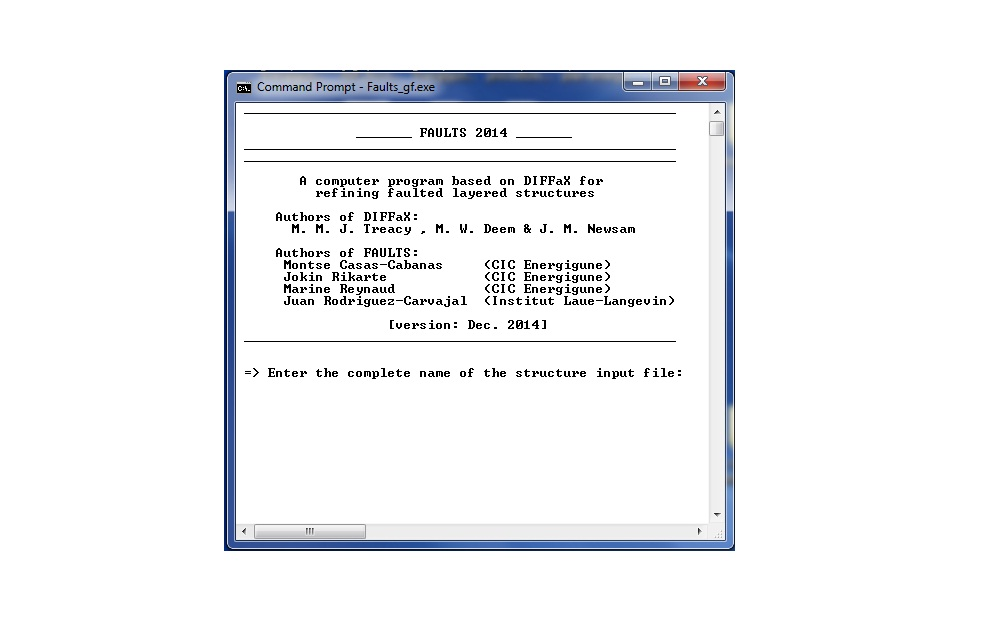
\includegraphics [width= 4 in]{faultslayout.jpg}
\caption{\bf  FAULTS layout when invoked}
\label{faultslayout}
\end{center}
\end{figure}

Once the user enters the name of file CFILE.flts, if a refinement is to be done, the layout of the program will appear as in figure \ref{layout2}.
During the refinement process, depending on the option chosen by the user (see the comments on keyword \textit{Nprint} in the \textit{Calculation} subsection page \pageref{nprint}), the terminal will display the values of agreement factors at the end of each evaluation, and optionally the list of previous and new refinable parameters at each evaluation step.

 \begin{figure}[hbtp]
\begin{center}
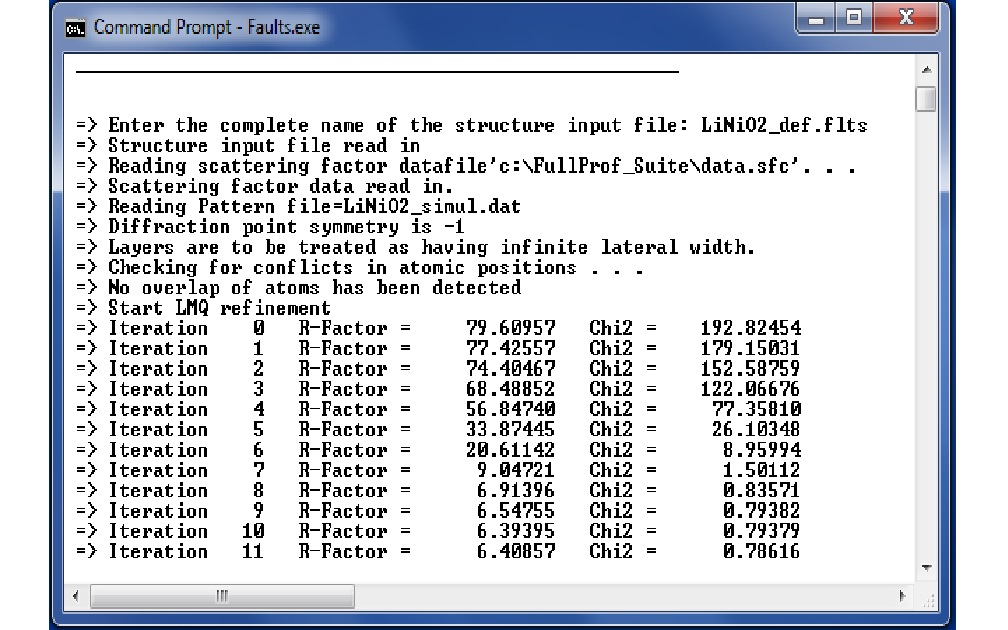
\includegraphics [width= 4 in]{faultslayout2.jpg}
\caption{\bf  FAULTS layout during refinement}
\label{layout2}
\end{center}
\end{figure}


Once the refinement has finished, the list of the best values obtained for the refinable parameters is displayed (see figure \ref{end}). The user can then open the CFILEn.prf to see the goodness of the refinement.


\begin{sidewaysfigure}[h!]
\begin{center}
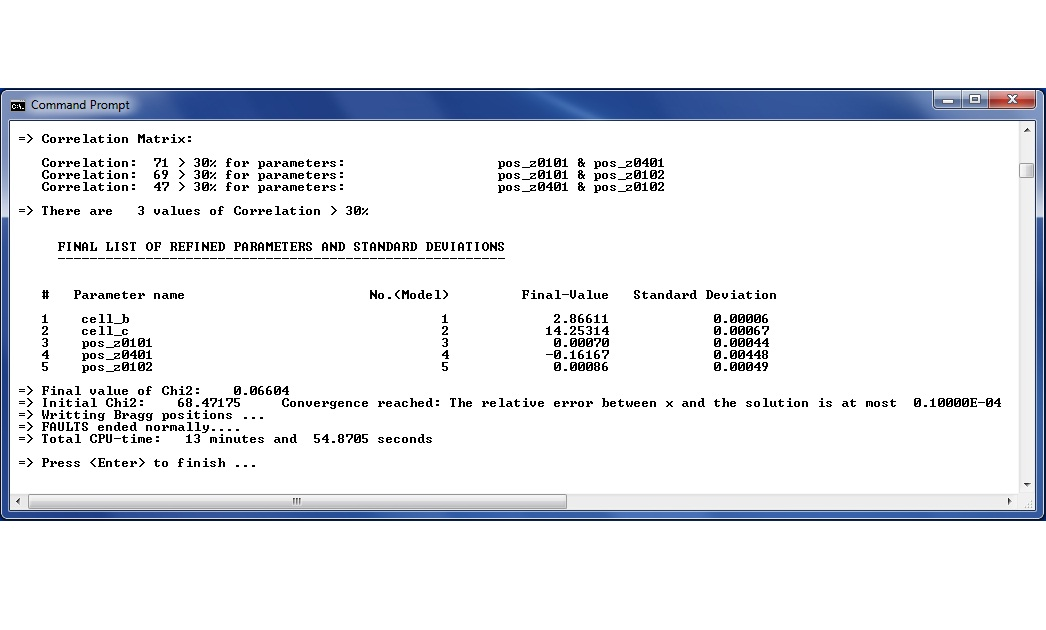
\includegraphics [width= 7.0 in]{faultsend.jpg}
\caption{\bf  FAULTS layout at the end of the refinement}
\label{end}
\end{center}
\end{sidewaysfigure}

 }

\chapter{Example}
\label{example}







\section{Stacking faults in LiNiO$_{2}$}

Lithium nickel oxide has been intensively studied as a positive electrode material in Li-ion batteries \cite{Whit2004}.
As other lithium transition metal oxides, it crystallizes in an O3-type layered structure consisting in three NiO$_{2}$ slabs per unit cell, with an ABCABC oxygen stacking sequence, and lithium ions located in the octahedral sites of the interlayer spaces (see figure \ref{estructura}). In order to explain the significant broadening of the (10\emph{l}) and (01\emph{l}) diffraction lines, DIFFaX simulations have been used for this material with the hypothesis of the existence of O1 stacking faults in the structure at low lithium concentrations (Li$_{\epsilon}$Ni$_{1.02}$O$_{2}$, $\epsilon\leq$ 0.3) \cite{Crog2000}. These stacking faults represent a break in the normal stacking sequence of the structure, with a local ABAB oxygen stacking sequence.

\begin{figure}[h!]
\begin{center}
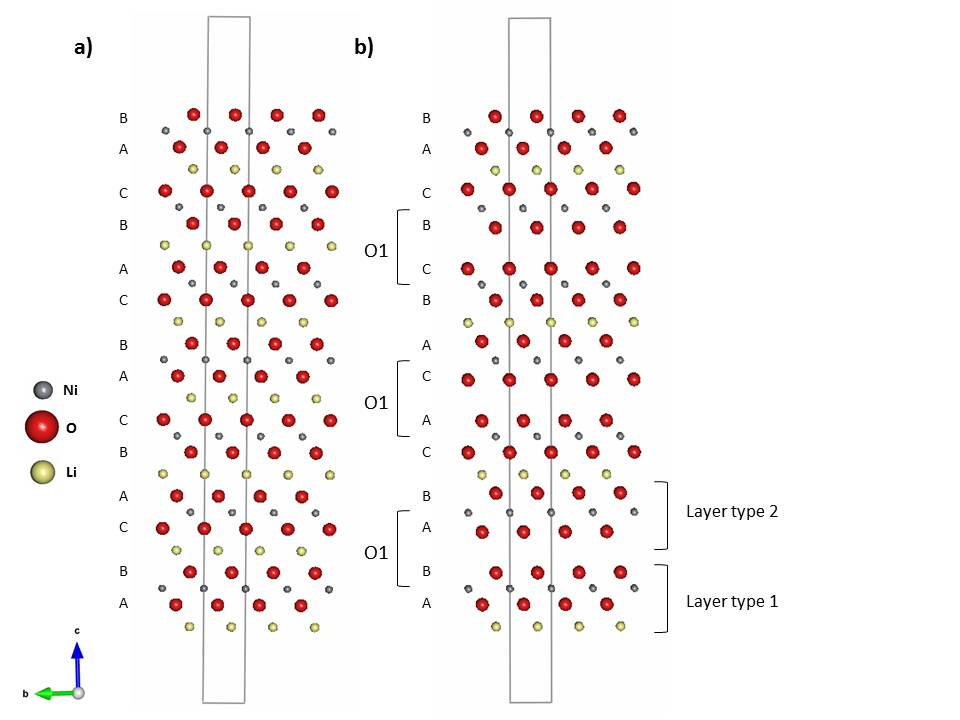
\includegraphics [width=5.3 in]{LiNO_estructura.jpg}
\caption{\bf a) Ideal structure of lithium nickel oxide (LiNiO$_{2}$) with O3 stacking, and b) defective structure with O1 stacking faults (Li$_{\epsilon}$Ni$_{1.02}$O$_{2}$).}
\label{estructura}
\end{center}
\end{figure}

The ideal structure can be described with three layers, each one containing a NiO$_{2}$ slab and a lithium interslab. The three layers are structurally identical, but shifted with respect to each other, resulting in transition vectors $\vec{t}_{12}$=$\vec{t}_{23}$=$\vec{t}_{31}$=(2/3 1/3 1/3) and a stacking probability of 1 for each transition. O1 defects require the definition of a new type of layer, structurally different, since these defective layers do not contain any lithium (see figure \ref{esquemacapes}). Therefore, three more layers are defined in the faulted structure, structurally identical between each other but different from the previous ones, and new transitions are allowed  in order to describe the defects (see figure \ref{capes}).

\begin{sidewaysfigure}
\begin{center}
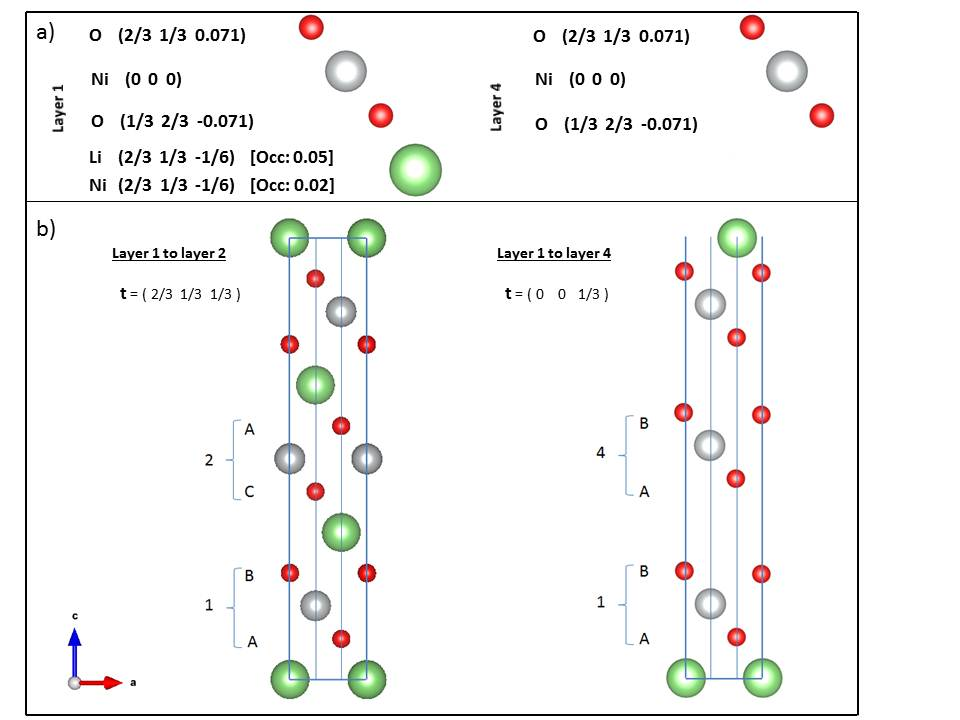
\includegraphics [width=6in]{description.jpg}
\caption{\bf  a) Schematic representation and atomic coordinates of the layers required for describing stacking faults for Li$_{0.05}$Ni$_{1.02}$O$_{2}$ in the FAULTS program. b) Graphic representation of the different transition possibilities from layer 1 and transition vectors.}
\label{esquemacapes}
\end{center}
\end{sidewaysfigure}

\begin{figure}[h!]
\begin{center}
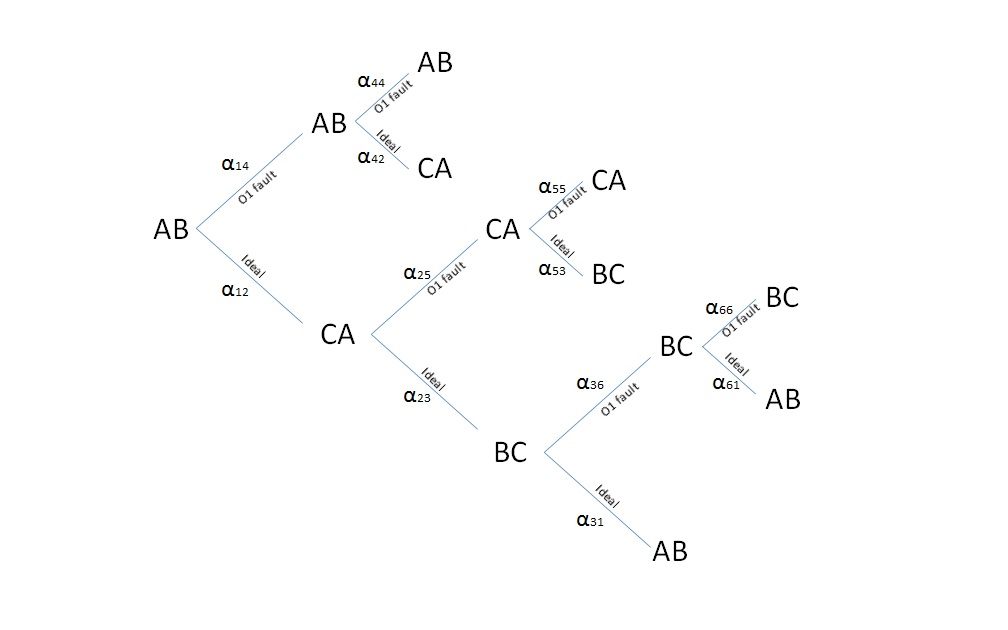
\includegraphics [width=5.2 in]{transitions.jpg}
\caption{\bf Possible layer transitions for Li$_{\epsilon}$Ni$_{1.02}$O$_{2}$ containing O1-type stacking faults, where $\alpha_{ij}$ is the probability transition from layer \emph{i} to layer \emph{j}.}
\label{capes}
\end{center}
\end{figure}





\section{Analysis of simulated data}
\label{Analysis of simulated data}

By  means of the  stacking description described above, FAULTS has been used to simulate a diffraction pattern with the parameter's values described in table \ref{taulasim}.
The obtained simulated XRD pattern for Li$_{\epsilon}$Ni$_{1.02}$O$_{2}$ ($\epsilon\leq$ 0.3) has then been used to analyse and test out the program. This are also the example files (LiNiO2$\_$simul.flts and LiNiO2$\_$refine.flts) included with the program. The refinement has been done by means of the Levenberg Marquart minimization algorithm, restraining the program to a maximum of 2400 function evaluations and a criterion of convergence 0.1e-4. As an example of the refinement process, the initial values of the refined parameters, which have been chosen far enough from the correct ones not to bias the result,
and  the final refined values are also  shown in table \ref{taulasim}.
A visual comparison between the calculated and the simulated powder patterns and their difference is shown in figure \ref{sim}.
Starting Rp and Chi$^{2}$ values were 45.62$\%$  and 186.38 respectively and reached a final value of 4.86$\%$ and 1.03 respectively.
The values of the refined parameters are very close to those used in the simulation and lead to a XRD pattern practically
identical to the one obtained with the values of these parameters used in the simulation (see figure \ref{sim}).



\begin{table}
\begin{center}
\begin{tabular}{|c|c|c|c|}
\hline
Refined parameter & Simulation & Initial value & Final value(Std dev.)\\

\hline
a,b & 2.81540 & 2.86540 & 2.81510(10)\\
\hline
c & 13.363000 & 13.26300 & 13.3638(7)\\
\hline
Scale & 1.00000 & 1.00000 & 1.010(3)\\
\hline
z$_{O1}$,z$_{O3}$ & 0.07133	&0.17133&	0.0716(2)\\
\hline
z$_{O2}$,z$_{O4}$ & -0.07133	&-0.17133& -0.0716(2)\\
\hline
$\alpha_{12}$,$\alpha_{23}$,$\alpha_{31}$ & 0.8580&	1.0000	&0.8569(10)\\
\hline
$\alpha_{14}$,$\alpha_{25}$,$\alpha_{36}$ & 0.1420&	0.0000	&0.1431(10)\\
\hline
$\alpha_{42}$,$\alpha_{53}$,$\alpha_{61}$ & 0.8580&	1.0000	&0.842(6)\\
\hline
$\alpha_{44}$,$\alpha_{55}$,$\alpha_{66}$ & 0.1420&	0.0000	&0.158(6)\\
\hline


\end{tabular}
\caption{\textbf{Starting and final values of the parameters refined in the analysis of simulated data.}}
\label{taulasim}
\end{center}
\end{table}


\begin{sidewaysfigure}
\begin{center}
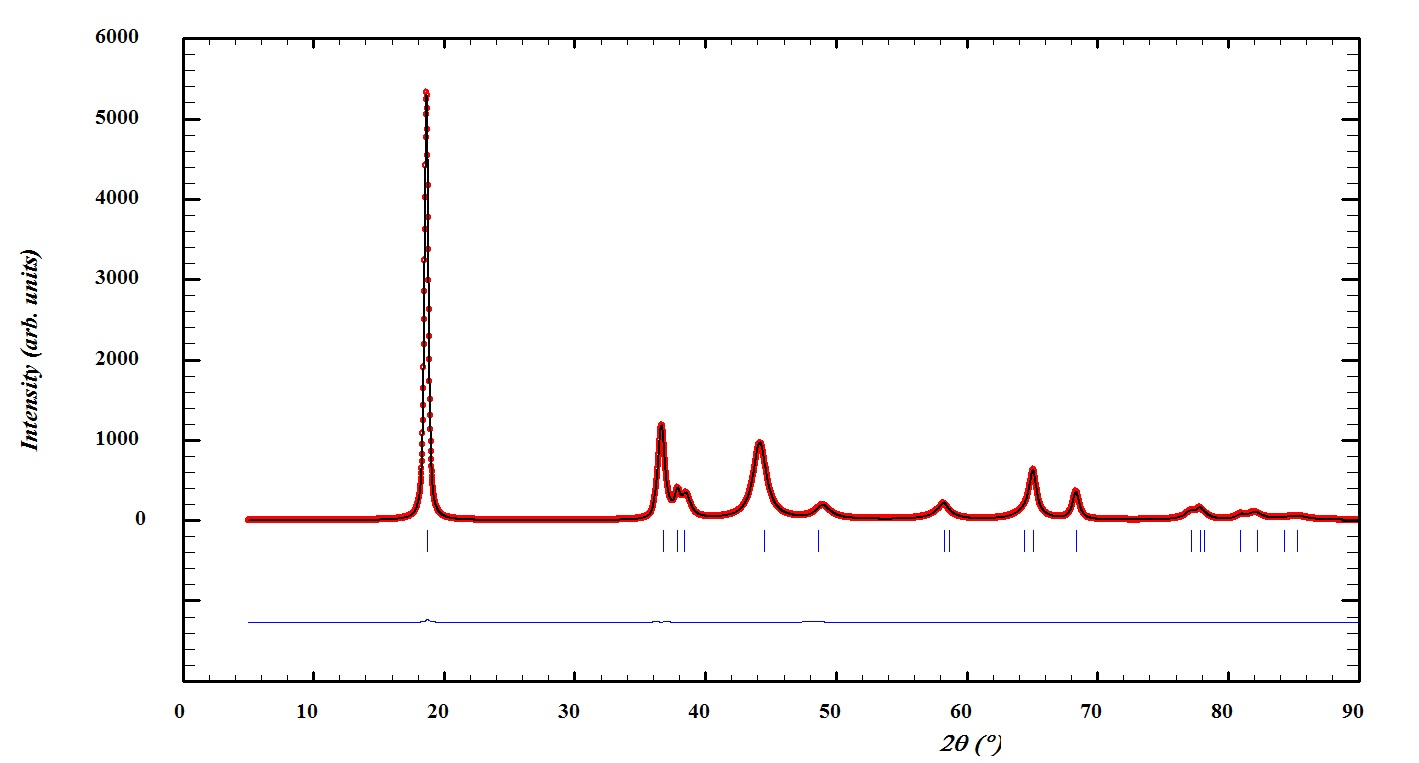
\includegraphics [width=6 in]{pattern.jpg}
\caption{\bf Comparison of the X-ray diffraction patterns corresponding to the FAULTS analysis of the simulated data: simulated pattern (dotted curve) and calculated pattern using the FAULTS refinement (continuous curve). The diagram underneath shows the difference between them. The ticks show the position of the Bragg reflections of the R-3m average unit cell (the one used to describe the ideal O3 structure of Li$_{\epsilon}$Ni$_{1.02}$O$_{2}$).  }
\label{sim}
\end{center}
\end{sidewaysfigure}

An example of the evolution of \textit{a} and \textit{b} cell parameters and of Chi$^{2}$ and Rp throughout a run of 12 iteration cycles is shown in \ref{cycles}.

\begin{figure}[!htbp]
\begin{center}
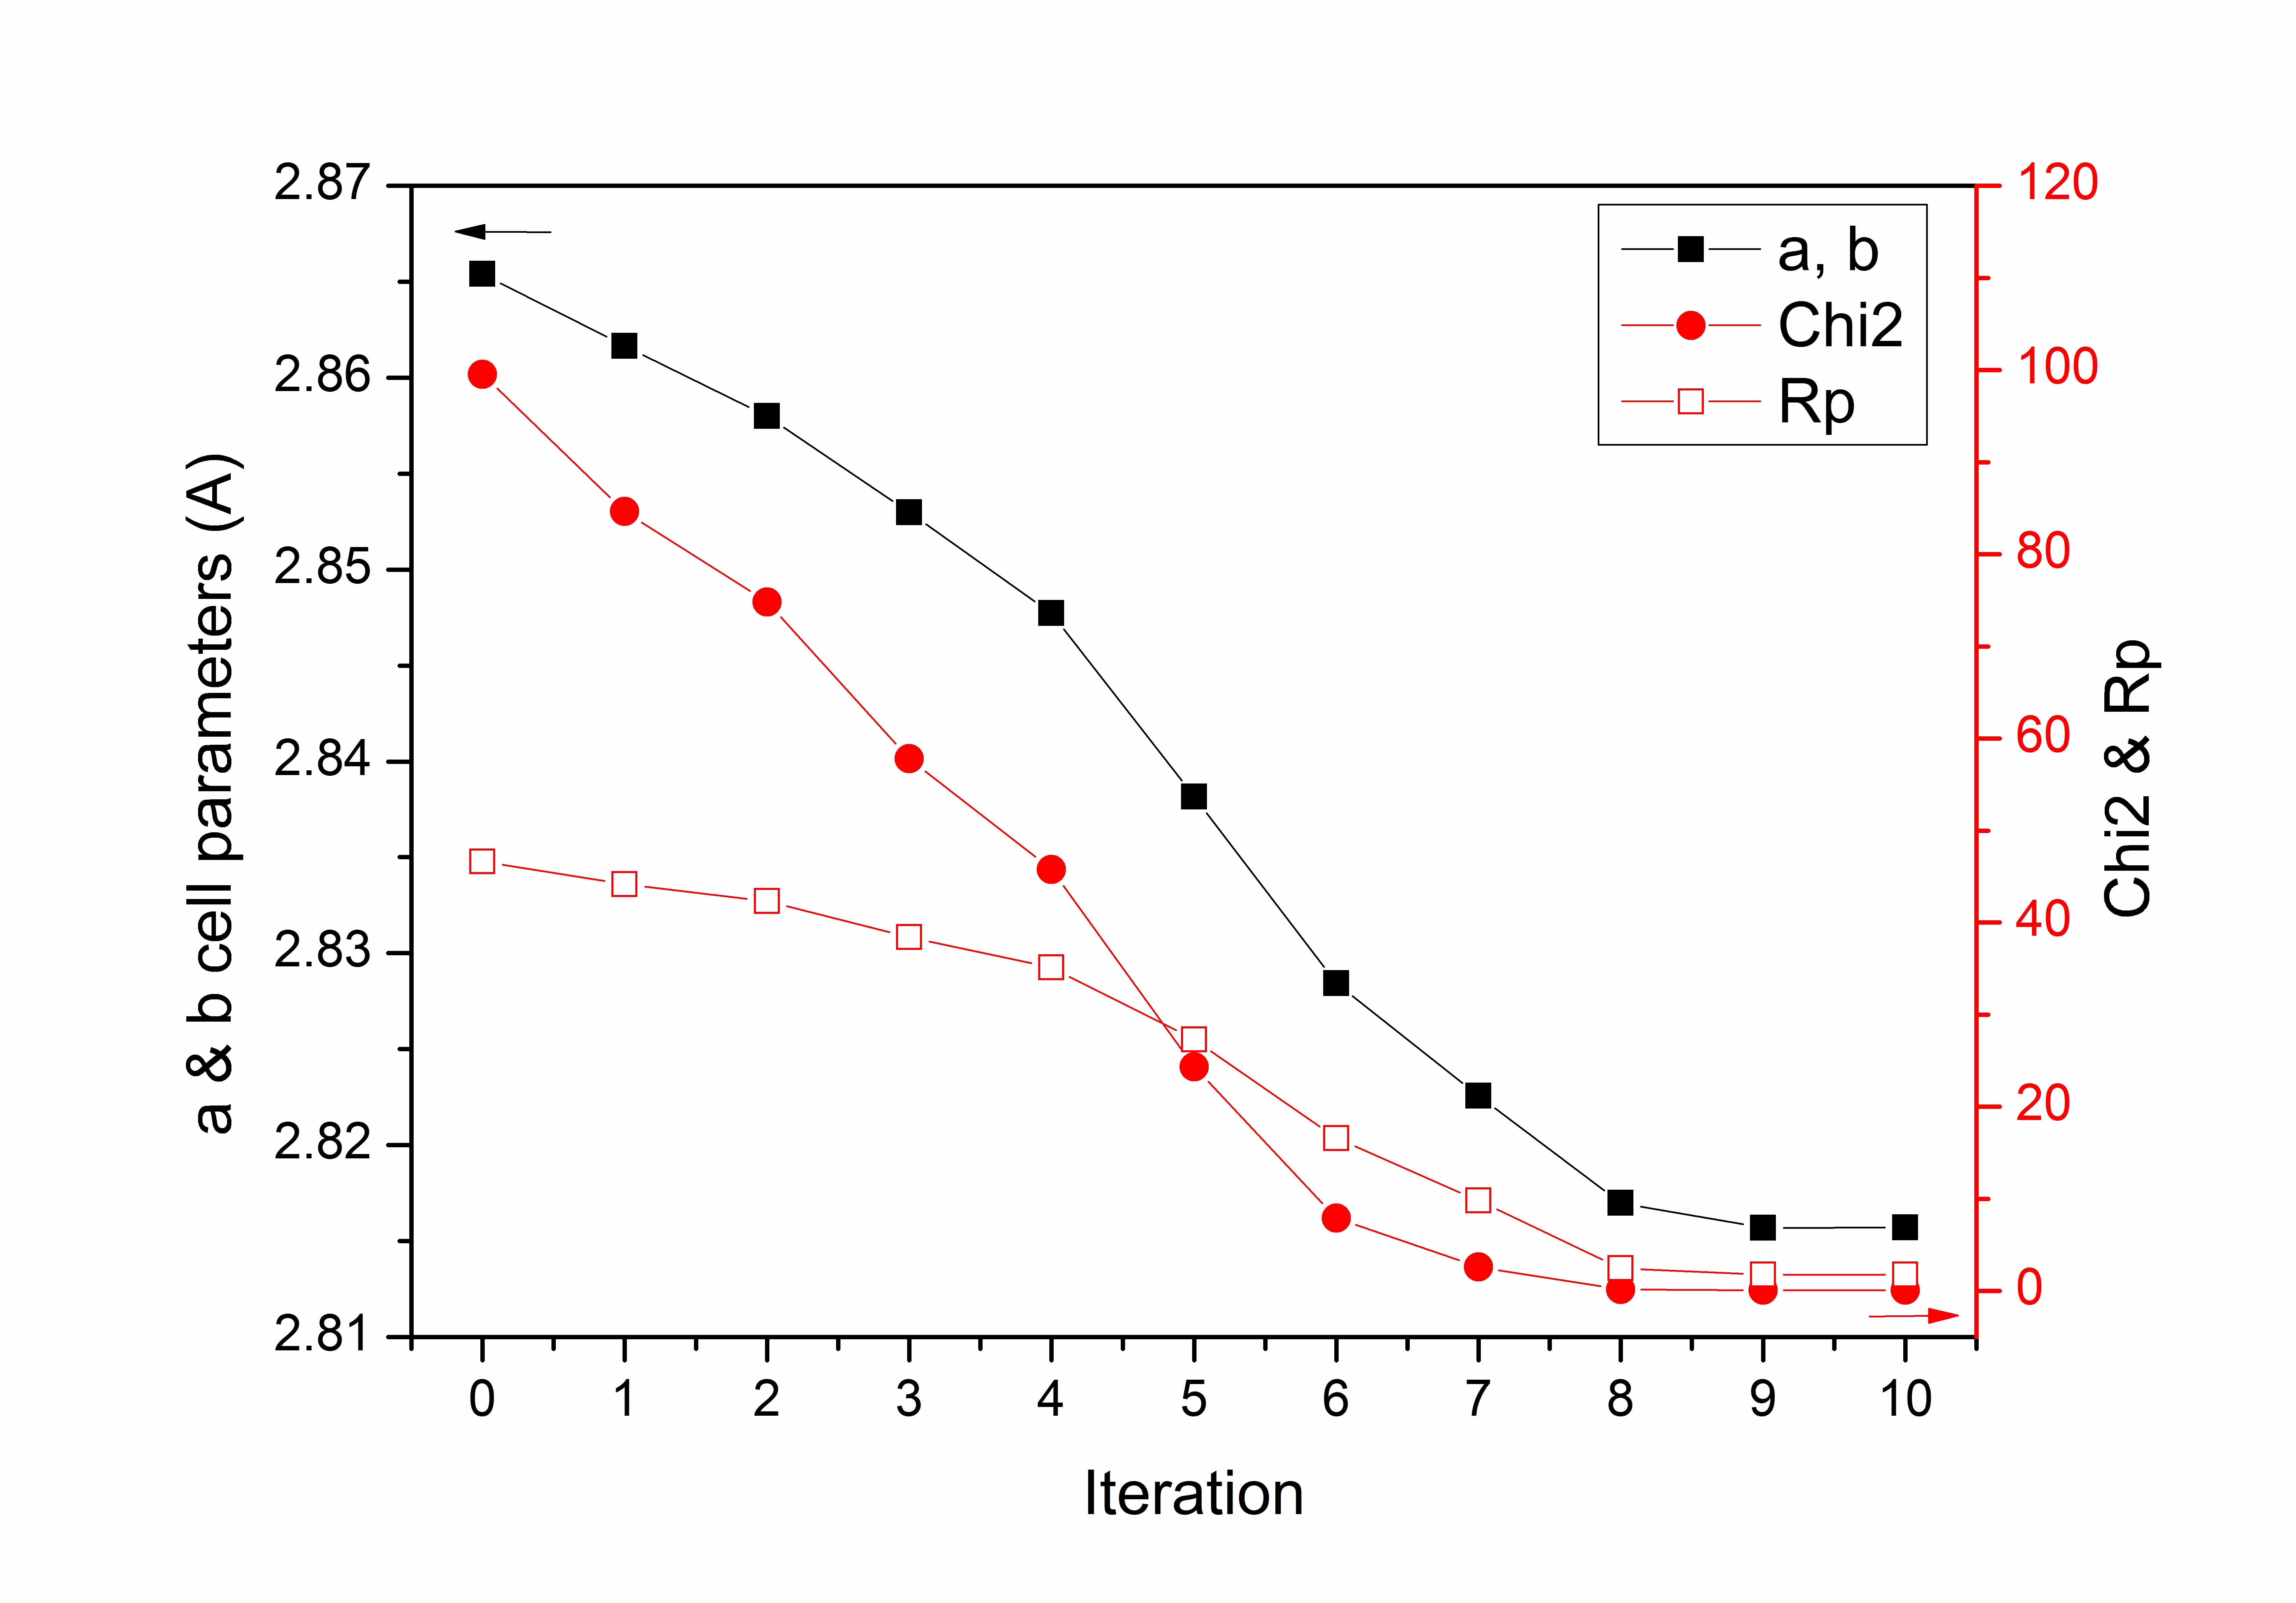
\includegraphics [width=4 in]{chi2_Rf.jpg}
\caption{\bf Evolution of the functions Rp and Chi$^{2}$ and of the cell parameters a and b, versus the cycle number. }
\label{cycles}
\end{center}
\end{figure}

\chapter{Frequent errors}
\label{freqerrors}



This part of the manual is a tentative of compiling frequent mistakes made by new users of FAULTS. This list is far from being exhaustive. It is only intended to help beginners in starting working correctly with FAULTS and doesn't dispense the user of a carefull reading of the entire manual. 
The authors would be grateful if users could notify them about other possible sources of errors not reported below or about possible bugs in the program (faults*at*cicenergigune.com or fullprof*at*ill.fr).\\

First of all, the users should always read carefully the messages written by FAULTS in the command window and in the output file .out. Most of the errors can be identified from these messages.\\


\section{Input control file .flts}

\begin{itemize}

	\item Tabs are not allowed in the input files of FAULTS. Only spaces can be used.

	\item All the non-optionnal sections and keywords have to be present in the .flts input file. 

	\item Contrary to the .pcr input files used in FullProf, a missing refinement code will not considered as zero but will produce an error, so all the refinement codes have to be present in the .flts input file. 

	\item Contrary to the .pcr input files used in FullProf, empty lines can be used in the .flts input file.

	\item The combination of the profile parameters U, V, W, X should not led to a profile function with negative values (no negative Gaussian and/or Lorentzian FWHM). The user can check this by calculating the Gaussian and and Lorentzian FWHM ($H_{G}^{2}$ and $H_{L}$) with the formula given page \pageref{FWHM} using the program  WinPLOTR \cite{WinplotrPaper, WinplotrWebsite} (Menu \emph{Calculations} $=$$>$ \emph{I.R.F. (U,V,W,X,Y,Z)}) or any spreadsheet.

\end{itemize}

\section{Input data files}

\begin{itemize}

	\item Make sure to comply with the description of each file type.

	\item No intensity can be zero o negative.

	\item Empty lines should be avoided.

\end{itemize}

\section{Other remarks}

\begin{itemize}

	\item The way of working with FAULTS requires especial care of the user. Before starting to do refinements it is advisable to make simulations in order to start with an initial model that is not too far from the experimental diffraction pattern. 
	
	\item If the structural model is complicated, the first calculations can take time, so the user should make sure that he/she lets the program some minutes before concluding that it is blocked. Keep in mind that the derivatives are calculated numerically by calling two times the total function per free parameter and this calculation may be expensive in CPU-time.

\end{itemize}
 






\pagenumbering{Roman}



\begin{thebibliography}{99}


\bibitem{DiffaxPaper} Treacy M.M.J., Newsam J.M. and Deem M.W. A general recursion method for calculating diffracted intensities from crystals containing planar faults. \textit{Proc. R. Soc. Lond. A}, 433:499-520, 1991. 

\bibitem{DiffaxDownload} Treacy M.M.J., Newsam J.M. and Deem M.W. DIFFaX. Available at: \url{http://www.public.asu.edu/~mtreacy/DIFFaX.html}. 

\bibitem{CrysFMLPaper} Rodr$\acute{\i}$guez-Carvajal J. and Gonzalez-Platas J., Crystallographic Fortran 90 modules library (CrysFML): a simple toolbox for crystallographic computing programs. \textit{IUCr CompComm. Newsletter}, 1:50-58, 2003. Available at: \url{http://www.iucr.org/iucr-top/comm/ccom/newsletters/}. 

\bibitem{CrysFMLDownload} Rodr$\acute{\i}$guez-Carvajal J. and Gonzalez-Platas J., CrysFML repository. Available at: \url{http://forge.epn-campus.eu/projects/crysfml/repository/}.

\bibitem{DiffaxMaths} Treacy M.M.J., Deem M.W., and Newsam J.M. DIFFaX Manual, 2005, Chap 8: How DIFFaX works (p48). Available at: \url{http://www.public.asu.edu/~mtreacy/DIFFaX$\_$manual.pdf}. 

\bibitem{Hend1942} Hendricks S. and Teller E. X-ray interference in partially ordered layer lattices. \textit{J. Chem. Phys.}, 10:147-167, 1942.

\bibitem{FAULTSPaper1} Casas-Cabanas M., Rodr$\acute{\i}$guez-Carvajal J., Palac$\acute{\i}$n M.R., \textit{Z. Kristallogr. Suppl.}, 23:243-248, 2006. 

\bibitem{FAULTSPaper2} Casas-Cabanas M., Rikarte Ormazabal J., Reynaud M., Rodr$\acute{\i}$guez-Carvajal J., \textit{in preparation}.

\bibitem{FPDownload} Rodr$\acute{\i}$guez Carvajal J., FullProf Suite. Available at: \url{http://www.ill.eu/sites/fullprof}.

\bibitem{FPPaper} Rodr$\acute{\i}$guez Carvajal J., Physica B.(1993), 192, Recent advances in magnetic structure determination by neutron powder 
diffraction. \textit{Physica B.}, 192:55-69, 1993.

\bibitem{FPManual} Rodr$\acute{\i}$guez Carvajal J., FullProf Manual. Available at \url{http://www.ill.eu/sites/fullprof/php/tutorials.html}.

\bibitem{DiffaxManual} Treacy M.M.J., Deem M.W., and Newsam J.M. DIFFaX Manual, 2005. Available at: \url{http://www.public.asu.edu/~mtreacy/DIFFaX$\_$manual.pdf}. 

\bibitem{FPSDownload} Rodr$\acute{\i}$guez Carvajal J. and Chapon L., FullProf Studio. Available at \url{http://www.ill.eu/sites/fullprof/index.html}.

\bibitem{FPSManual} Rodr$\acute{\i}$guez Carvajal J. and Chapon L., FullProf Studio Manual. Available at \url{http://www.ill.eu/sites/fullprof/index.html}.

\bibitem{VESTApaper} Momma K. and Izumi F. VESTA3 for three-dimensional vizualization of crystal, volumetric and morphology data. \textit{Journal of Applied Crystallography}, 44:1272-1276, 2011.

\bibitem{VESTAwebsite} Momma K. and Izumi F., VESTA (Visualization for Electronic and STrcutural Analysis). Available at \url{http://jp-minerals.org/vesta/en/}.

\bibitem{imageJ} \url{http://imagej.nih.gov/ij/index.html}

\bibitem{WinplotrPaper} Roisnel T. and Rodr$\acute{\i}$guez Carvajal J., WinPLOTR: A windows tool for powder diffraction pattern analysis. \textit{Mater Sci Forum}, 378(3):128-123, 2000.

\bibitem{Whit2004} Whittingham M. S., Lithium Batteries and Cathode Materials. \textit{Chemical Reviews}, 104:4271-4301, 2004. 

\bibitem{Crog2000} Croguennec L., Pouillerie C., Mansour A. N. and Delmas C., Structural characterisation of the highly deintercalated Li$_{x}$Ni$_{1.02}$O$_{2}$ phases (with x$\leq$0.30). \textit{Journal of Materials Chemistry}, 11:131-141, 2000.



\end{thebibliography}

%-----------------------------------------------------------
%\addcontentsline{toc}{chapter}{\numberline{}Bibliography}
%\bibliography{biblioni}
%\bibliographystyle{unsrt}
%\include{biblio}
%-----------------------------------------------------------
\end{document}

